\documentclass[submission,copyright,creativecommons]{eptcs}
\providecommand{\event}{SYNT 2018} % Name of the event you are submitting to

\usepackage{bookmark}
\usepackage{underscore}
\usepackage{graphicx}
\usepackage{adjustbox}
\usepackage{array}
\usepackage{booktabs}
\usepackage{caption}    % for side-by-side figures
\usepackage{subcaption} % for side-by-side figures
\usepackage{multirow}

\usepackage{tikz}
\def\checkmark{\tikz\fill[scale=0.4](0,.35) -- (.25,0) -- (1,.7) -- (.25,.15) -- cycle;} 

\usepackage[inline]{enumitem}
\newcommand{\inliststyle}[1]{\textbf{\smaller#1}}
\newlist{inlist}{enumerate*}{1}
\setlist[inlist]{label={\inliststyle{(\arabic*)}}}

\title{SyGuS-Comp 2018: Results and Analysis}
\author{
	Rajeev Alur 
	\institute{University of Pennsylvania}
  \and
	Dana Fisman
	\institute{Ben-Gurion University}
  \and
	Saswat Padhi
	\institute{University of California, Los Angeles}
  \and
	Rishabh Singh
	\institute{Google Brain}
  \and
	Abhishek Udupa
	\institute{Microsoft, Redmond}
}
\def\titlerunning{SyGuS-Comp 2018: Results and Analysis}
\def\authorrunning{R. Alur, D. Fisman, S. Padhi, R. Singh \& A. Udupa}
\def\copyrightholders{Alur, Fisman, Padhi, Singh \& Udupa}
\begin{document}
\maketitle

%%%%%%%%%%%%%%% MACROS %%%%%%%%%%%%%%

\newcommand{\alc}{\textsc{Alchemist-cs}}
\newcommand{\alccsdt}{\textsc{Alchemist-csdt}}
\newcommand{\cvc}{\textsc{CVC4}}
\newcommand{\cvclast}{\ensuremath{\textsc{CVC4}_{2017}}}
\newcommand{\enum}{\textsc{Enumerative}}
\newcommand{\skac}{\textsc{Sketch-ac}}
\newcommand{\ice}{\textsc{Ice-dt}}
\newcommand{\toast}{\textsc{SosyToast}}
\newcommand{\stoch}{\textsc{Stochastic}}
\newcommand{\cvcnew}{\ensuremath{\textsc{CVC4}_{2018}}}
\newcommand{\eusolver}{\textsc{EUSolver}}
\newcommand{\eusolverlast}{\ensuremath{\textsc{EUSolver}_{2016}}}
\newcommand{\eusolvernew}{\ensuremath{\textsc{EUSolver}_{2017}}}
\newcommand{\euphony}{\textsc{Euphony}}
\newcommand{\ethree}{\textsc{e3solver}}
\newcommand{\dryd}{\textsc{DryadSynth}}
\newcommand{\lig}{\textsc{LoopInvGen}}
\newcommand{\sygus}{SyGuS}
\newcommand{\comp}{SyGuS-Comp}

\newcolumntype{R}[2]{%
	>{\adjustbox{angle=#1,lap=\width-(#2)}\bgroup}%
	l%
	<{\egroup}%
}
\newcommand*\rot{\multicolumn{1}{R{90}{1em}}}% no optional argument here, please!

\newcommand{\verify}[1]{\textcolor{red}{#1}}

%%%%%%%%%%%%%%%%%%%%%%%%%%%%%%%%%%%%%

\begin{abstract}
    \emph{Syntax-Guided Synthesis (SyGuS)} is the computational problem of finding an implementation $f$
    that meets both a semantic constraint given by a logical formula $\varphi$ in a background theory $T$,
    and a syntactic constraint given by a grammar $G$,
    which specifies the allowed set of candidate implementations.
    Such a synthesis problem can be formally defined in the SyGuS Input Format (SyGuS-IF),
    a language that is built on top of SMT-LIB.
    
    
    The \emph{Syntax-Guided Synthesis Competition (\comp)} is an
    effort to facilitate, bring together and accelerate research and development of efficient
    solvers for SyGuS by providing a platform for evaluating different synthesis
    techniques on a comprehensive set of benchmarks. 
    In this year's competition, five solvers competed on over 1600 benchmarks.
    This paper presents and analyses the results of the 5\textsuperscript{th} \comp{} held in 2018.
\end{abstract}

%\section{Introduction}
%\label{sec:intro}

The \emph{Syntax-Guided Synthesis Competition} (SyGuS-Comp) is an annual competition aimed to provide an objective platform for comparing different approaches for solving the \emph{Syntax-Guided Synthesis} (SyGuS) problem. A SyGuS problem takes as input a logical specification $\varphi$ for what a synthesized function $f$ should compute, and a grammar $G$ providing syntactic restrictions on the function $f$ to be synthesized. Formally, a solution to a SyGuS instance $(\varphi,G,f)$ is a function $f_{imp}$ that is expressible in the grammar $G$ such that the formula $\varphi[f/f_{imp}]$ obtained by replacing  $f$ by $f_{imp}$ in the logical specification $\varphi$ is valid. SyGuS instances are formulated in SyGuS-IF~\cite{RaghothamanU14}, a format built on top of SMT-LIB2~\cite{smtlib}.

We report here on the 4th SyGuS competition that took place in July 2017, in Heidelberg, Germany as a satellite event of CAV'17 (The 29th International Conference on Computer Aided Verification) and SYNT'17 (The Sixth Workshop on Synthesis). As in the previous competition there were four tracks: the general track, the conditional linear integer arithmetic track, the invariant synthesis track, and the programming by examples track. We assume most readers of this report are already familiar with the SyGuS problem and the tracks of SyGuS-Comp and thus refer the unfamiliar reader to the report on last year's competition~\cite{SyGuSComp15}. 

The report is organized as follows. Section~\ref{sec:benchs} describes the participating benchmarks. Section~\ref{sec:solvers}  lists the participating solvers, and briefly describes the main idea behind their strategy.  Section~\ref{sec:exp-set} provides details on the experimental setup. Section~\ref{sec:comp-results} gives an overview of the results per track. Section~\ref{sec:benchs-pres} provides details on the results, given from a single benchmark respective. Section~\ref{sec:discussion} concludes.
\section{Participating Benchmarks}
\label{sec:benchs}

In addition to last year's benchmarks, we received 4 new sets of benchmarks this year, which are shown in Table~\ref{tbl:new-benchmarks}. 


\paragraph{Program Repair}
The 18 program repair benchmarks correspond to the task of generating small expression repairs that are consistent with a given set of input-output examples~\cite{repairbenchmarks}. These benchmarks were extracted from real-world Java bugs by manually analyzing the developer commits that involved changes to fewer than 5 lines of code. The key idea of the program repair approach is to the first localize the fault location in a buggy program and generate the corresponding input-output example behavior for the buggy expression from passing test cases. In the second phase, the task of repairing the buggy expression can be framed as a SyGuS problem, where the goal is to synthesize an expression that comes from a family of expressions defined using a context-free grammar of expressions and that satisfies the input-output example constraints.

\paragraph{Crypto Circuits}
The Crypto Circuits benchmarks comprise of tasks of synthesizing constant-time circuits that are cryptographically resilient to timing attacks~\cite{EldibWW16}. Consider a circuit $C$ with a set of \emph{private} inputs $I_0$ and a set of \emph{public} inputs $I_1$ such that if an attacker changes the values of
the public inputs and observes the corresponding output, she is unable to infer the values
of the private inputs (under standard assumptions about computational resources in cryptography). An attacker can gain information about private inputs by analyzing the time the circuit takes to compute the output values on public inputs, e.g. when a public input bit changes from 1 to 0, a specific output bit is guaranteed to
change from 1 to 0 independent of whether a particular private input bit is 0 or 1, but 
may change faster when this private input is 0, thus leaking information.
The timing attack can be prevented if the circuit satisfies the \emph{constant-time} property:
A constant-time circuit is the one in which the length of all input-to-output paths  measured in terms of number of gates
are the same.

The problem of synthesizing a new circuit $C'$ that is functionally equivalent to a given circuit $C$ such that $C'$ is a constant-time circuit can be formalized as a SyGuS problem. A context-free grammar can be used to define the set of all constant-time circuits with all input-to-output path lengths within a given bound, and the functional equivalence constraint can be expressed as a Boolean formula~\cite{EldibWW16}.

\paragraph{Instruction Selection}
The Instruction Selection benchmarks consist of tasks for synthesizing a ``Bit Test and Reset" instruction from the set of basic bitvector operations, in a way similar to the implementations supported by the x86 processors. These benchmarks comprise of 4 different addressing variants with increasing levels of complexity:
\begin{itemize}
	\item btr*: Read from register.
	\item btr-am-base*: Load from memory address base.
	\item btr-am-base-index*: Load from memory address base with indexing.
	\item btr-am-base-index-scale-disp*:  Load from memory address base with index shifted with scale.
\end{itemize}

\paragraph{Invariant Generation}
The invariant generation benchmarks comprise of the task of generating a loop invariant (as a conditional linear arithmetic expression) given the pre-condition, post-condition and the transition function corresponding to the loop body. The 7 new benchmarks~\cite{PadhiM17} correspond to loop invariant tasks adapted from several recent invariant inference papers including generating path invariants, abductive inference, and NECLA Static analysis benchmarks.


\begin{table}
	{\small{
			\begin{center}
				\scalebox{0.94}{
				\begin{tabular}{rcl}
					Benchmark Set &  \# of benchmarks &  Contributors \\ \hline \hline
					Invariant Generation & 7 & Saswat Padhi (UCLA)  \\
					Program Repair & 18 & 	Xuan Bach D Le (SMU), David Lo (SMU) and Claire Le Goues (CMU) \\
					Crypto Circuits & 214 & Chao Wang (USC) \\		
					Instruction Selection & 28 & Sebastian Buchwald (KIT) and Andreas Fried (KIT) \\
				\end{tabular}
			}
			\end{center}
			\caption{New Contributed Benchmarks}
			\label{tbl:new-benchmarks}
		}}
	\end{table}
\section{Participating Solvers}
\label{sec:solvers}

Six solvers were submitted to this year's competition. \eusolvernew, an improved version of \eusolver;  \cvcnew, an improved version of \cvc; \euphony, a solver built on top of \eusolver; \dryd, a solver specialized for conditional linear integer arithmetic;  \lig, a solver specialized for invariant generation problems; and \ethree, a solver specialized for the bitvector category of the PBE track, built on top of the enumerative solver.
Table~\ref{tbl:solvers-authors} lists the submitted solvers together with their authors, and Table~\ref{tbl:solvers-in-tracks} summarizes which solver participated in which track.

\begin{table}[b]
	{\small{
			\begin{center}
				\scalebox{0.94}{
				\begin{tabular}{r||l}
					Solver &  Authors \\ \hline \hline
					\eusolvernew  	& Arjun Radhakrishna (Microsoft) and
					Abhishek Udupa (Microsoft) \\
					\cvcnew 		& Andrew Reynolds (Univ. Of Iowa),
					Cesare Tinelli (Univ. of Iowa), and 
					Clark Barrett (Stanford)  \\
					\euphony        & Woosuk Lee (Penn), Arjun Radhakrishna (Microsft) and Abhishek Udupa (Microsoft) \\
					\dryd           & Kangjing Huang (Purdue Univ.), Xiaokang Qiu (Purdue Univ.), and Yanjun Wang (Purdue Univ.)\\
					\lig            & Saswat Padhi (UCLA) and Todd Millstein (UCLA)\\
					\ethree         & Ammar Ben Khadra (University of Kaiserslautern)			
					\\
				\end{tabular}}
			\end{center}
			\caption{Submitted Solvers }
			\label{tbl:solvers-authors}
		}}
\end{table}


\begin{table}[t]
	\begin{center}
		\begin{tabular}{r||rrrrrr}
			& \multicolumn{6}{c}{Solvers} \\
			Tracks & \rot{\eusolvernew} & \rot{\cvcnew} & \rot{\euphony} & \rot{\dryd} & \rot{\lig} & \rot{\ethree} \\ \hline \hline
			LIA         & 1 & 1 & 1 & 1 & 0 & 0 \\
			INV         & 1 & 1 & 1 & 1 & 1 & 0\\
			General     & 1 & 1 & 1 & 0 & 0 & 0\\ 
			PBE Strings & 1 & 1 & 1 & 0 & 0 & 0\\ 
			PBE BV      & 1 & 1 & 1 & 0 & 0 & 1
		\end{tabular}
	\end{center}
	\caption{Solvers participating in each track}
	\label{tbl:solvers-in-tracks}
\end{table}


 The \eusolvernew\ is based on the divide and conquer strategy~\cite{AlurCAV15}. The idea is to find different expressions that work correctly for different subsets of the input space, and unify them into a solution that works well for the entire space of inputs. The sub-expressions are typically found using enumeration techniques  and are then unified into the overall expression using machine learning methods for decision trees~\cite{AlurRU17}.

 The \cvcnew\ solver is based on an approach for program synthesis that is implemented inside an SMT solver~\cite{ReynoldsDKTB15}. This approach extracts solution functions from unsatisfiability proofs of the negated form of synthesis conjectures, and uses  counterexample-guided techniques for quantifier instantiation (CEGQI) that make finding such proofs practically feasible. \cvcnew\ also combines enumerative techniques, and symmetry breaking techniques~\cite{ReynoldsT17}. 
 
 The \euphony\ solver leverages statistical program models to accelerate the \eusolver. The underlying statistical model is called probabilistic higher-order grammar (PHOG), a generalization of probabilistic context-free grammars (PCFGs). The idea is to use existing benchmarks and the synthesized results to learn a weighted grammar, and give priority to candidates which are more likely according to the learned weighted grammar.

 The \dryd\ solver combines enumerative and symbolic techniques. It considers benchmarks in conditional linear integer arithmetic theory (LIA), and can therefore assume all have a solution in some pre-defined decision tree normal form. It then tries to first get the correct height of a normal form decision tree, and then tries to synthesize a solution of that height. It makes use of parallelization, using as many cores as are available, and of optimizations based on solutions of typical LIA SyGuS problems.  
 
 The \lig\ solver~\cite{PadhiM17} for invariant synthesis extends the data-driven approach to inferring sufficient loop invariants from a collection of program states~\cite{PadhiSM16}. Previous approaches to invariant synthesis were restricted to using a fixed set, or a fixed template for features, e.g., ICE-DT~\cite{ICEDT,GNMR16} requires the shape of constraints (such as octagonal) to be fixed apriori. Instead \lig\, starts with no initial features, and automatically grows the feature set as necessary using program synthesis techniques. It reduces the problem of loop invariant inference to a series of precondition inference problems and uses a Counterexample-Guided Inductive Synthesis (CEGIS) loop to revise the current candidate.
 
 The \ethree\ solver for PBE bitvector programs, is built on top of the enumerative solver~\cite{AlurBJMRSSSTU13,UdupaRDMMA13}. It improves on the original \enum\ solver by applying unification techniques~\cite{AlurCAV15} and avoiding calling an SMT solver, since on PBE tracks there are no semantic constraints other than the input-to-output examples which can be checked without invoking an SMT solver.

\section{Experimental Setup} 
\label{sec:exp-set}

The solvers were run on the StarExec platform~\cite{starexec} with a dedicated cluster of 12 nodes,
where each node consisted of two 4-core 2.4\,GHz Intel processors with 256\,GB RAM and 1\,TB hard-disk space.
The memory usage limit for each solver run was set to 128\,GB, and the wall-clock time limit is set to 3600 seconds
(thus, a solver that used all 4 cores could consume at most 14400 seconds of CPU time).
The solutions that the solvers produced were checked for both syntactic and semantic correctness.
That is, a first postprocessor checked that the produced expression adhered to the grammar specified in the given benchmark,
and if this check passes, a second postprocessor checked that the solution adhered to semantic constraints
given in the benchmark (by invoking an SMT solver).
\section{Results Overview}
\label{sec:comp-results}

The combined results for all tracks are summarized in \Cref{fig:combinedresults},
which shows the total number of benchmarks solved by each solver in various track.
We observe that \cvcnew\ solved the highest combined number of benchmarks,
and \eusolvernew\ solved almost as many.

\begin{figure}
	\centering
	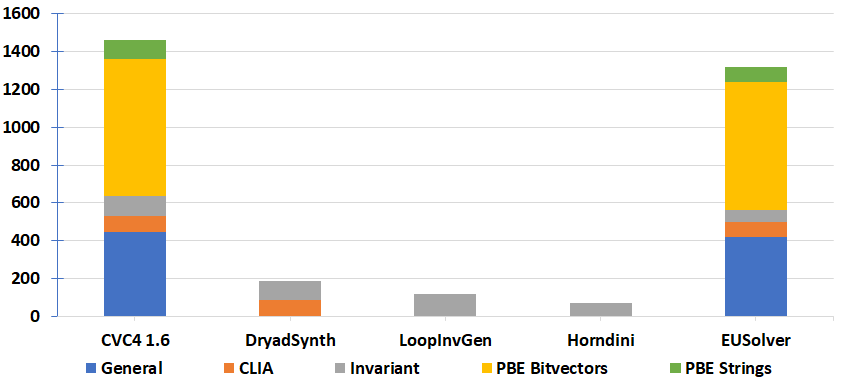
\includegraphics[width=0.95\textwidth]{figures/TotalSolved.png}
	\caption{The overall combined results for each solver on benchmarks from all five tracks.}
	\label{fig:combinedresults}
\end{figure}

The primary criterion for winning a track was the number of benchmarks solved,
but we also analyzed the time to solve and the the size of the generated expressions.
Both were classified using a pseudo-logarithmic scale as follows.
For time to solve, the scale is: $[0,1)$, $[1,3)$, $[3,10)$, $[10,30)$, $[30, 100)$,
$[100,300)$, $[300, 1000)$, $[1000,3600)$, $\geqslant 3600$.
That is, the first ``bucket'' refers to termination in less than one second,
the second to termination in one to three seconds and so on.
We say that a solver solved a certain benchmark \emph{among the fastest}
if the time it took to solve that benchmark is in the same bucket
as that of the solver which solved that benchmark in minimum time.
Similarly, for expression sizes, the pseudo-logarithmic scale we use is:
$[1,10)$, $[10,30)$, $[30,100)$, $[100,300)$, $[300,1000)$, $\geqslant 1000$,
where expression size is the number of nodes in the SyGuS parse-tree.
In some tracks there was a tie or almost a tie in terms of the number of solved benchmarks,
but the differences in the time to solve where significant.
We also report on the number of benchmarks \emph{solved uniquely} by a solver,
\emph{i.e.} the number of benchmarks which no other solver but this particular solver could solve.

\Cref{fig:resultsPerTrack} shows the percentage of benchmarks solved,
the percentage of those among the fastest,
and the percentage of synthesized expressions among the smallest size
for each solver in each track.

\begin{figure}
	\begin{center}
		\begin{minipage}{\textwidth}
			\centering
			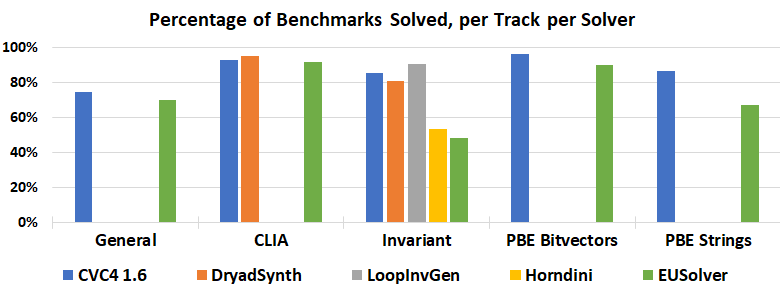
\includegraphics[width=0.95\textwidth]{figures/Solved.png}
		\end{minipage}
		\\[1cm]
		\begin{minipage}{\textwidth}
			\centering
			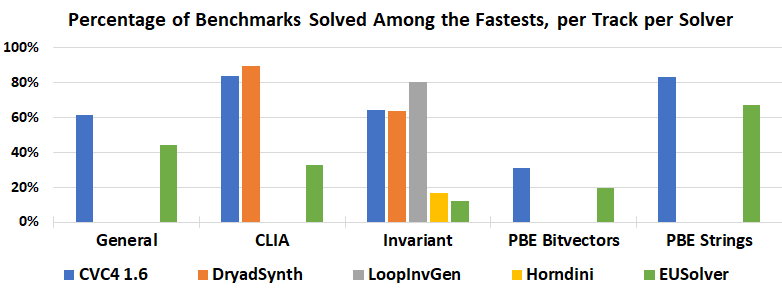
\includegraphics[width=\textwidth]{figures/Fastest.png}
		\end{minipage}
		\\[1cm]
		\begin{minipage}{\textwidth}
			\centering
			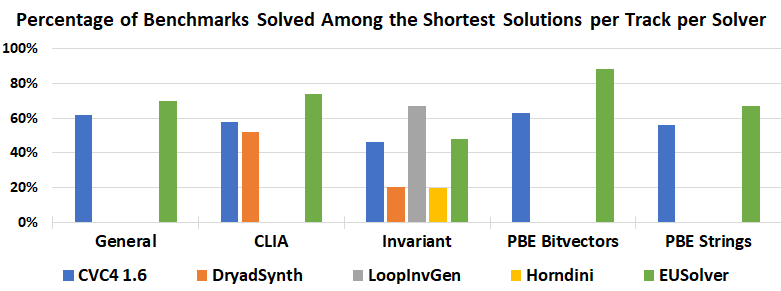
\includegraphics[width=\textwidth]{figures/Smallest.png}
		\end{minipage}
	\end{center}
	\caption{Percentage of benchmarks solved by different solvers across all tracks,
			 the percentage of benchmarks a solver solved among the fastest,
			 and the percentage of benchmarks for which the solver generated an expression among the smallest size.}
	\label{fig:resultsPerTrack}	
\end{figure}

\paragraph{General Track}
In the general track, \cvcnew\ solved more benchmarks than all others ($447$),
and \eusolvernew\ came second, solving $420$ benchmarks.
We note that the new version \cvcnew\ of \cvc, is significantly better than the previous version \cvclast,
which could only solve $395$ benchmarks.
The same order appears in the number of benchmarks solved among the fastest:
\cvcnew\ with 366, \eusolvernew\ with 266, and \cvclast\ with 231.
\verify{In terms of benchmarks solved uniquely by these solvers,
we have that \cvcnew\ solved ??? uniquely and \eusolvernew\ solved ??? uniquely.}

\begin{table}[t]
	\begin{center}
		\scalebox{0.9}{
		\begin{tabular}{lr||rrrrrrrrrrrr|r}
			 &	& \rot{Compiler Optimizations and Bit Vectors}	& \rot{Let and Motion Planning} &	\rot{Invariant Generation with Bounded Ints} &	\rot{Invariant Generation with Unbounded Ints} &	\rot{Multiple Functions}	& \rot{Arrays} &	\rot{Hackers Delight} &	\rot{Integers} &	\rot{Program Repair} &	\rot{ICFP} &	\rot{Cryptographic Circuits} &	\rot{Instruction Selection} & {Total}\\\hline \hline
\multicolumn{2}{l||}{Number of benchmarks}  & 32 & 30 & 28 & 28 & 32 & 31 & 44 & 34 & 18 & 50 & 214 & 28 & 569 \\ \hline			 
\multirow{3}{*}{Solved} & \eusolvernew\ &	16	& 10	& 24	&24 &	18	& 31	& 35 &	33 &	14 &	50& 	152& 	0 & 407 \\
& \cvcnew\ &	15	& 15	& 24	& 24	& 12	& 31 &	44& 	34&	14&	48&	117&	0 & 378 \\
& \euphony\	& 19	&10 &	24 &	24 &	18	& 31	& 44	& 33	& 14	& 50	& 95 &	0 & 362 \\ \hline
\multirow{3}{*}{Fastest} & \eusolvernew\ &	7	&2 	& 12	& 14	& 6	& 5	& 20	& 14 &	13 &	40	& 143 &	0 & 276\\
 & \cvcnew &	11 &	15 &	18	& 19	& 9	& 31 &	44	& 33	& 7& 	19	& 30	& 0 & 236 \\
& \euphony	& 16 &	2	& 8	& 13 &	13 &	4	& 27 &	14 &	9	& 29	& 0& 	0 & 135 \\ \hline
\multirow{3}{*}{Uniquely} & \eusolvernew\ &	0	& 0& 	0	& 0& 	0	& 0& 	0	& 0 &	0	& 0	& 34 &	0 & 34 \\
& \cvcnew &	1	& 5&	0&	0&	1&	0	&0&	1&	1&	0	&0&	0 & 9\\
& \euphony	& 2	& 0	& 0& 	0	& 0& 	0	& 0& 	0	& 0& 	0 &	0	& 0 & 2\\ \hline			
		\end{tabular}}
	\end{center}
	\caption{\verify{Solvers performance across all categories of the general track}}
	\label{tbl:general-categories}
\end{table}

\verify{We partition the benchmarks of the general track according to categories where different categories consists of related benchmarks.
The results per category are given in the Table~\ref{tbl:general-categories}.
We can see that \eusolvernew\ preformed better than others in the categories of program repair, icfp and cryptographic circuits.
The \cvcnew\ solver preformed better than others in the categories of let and motion planning, invariant generation with bounded and unbounded integers,
arrays, integers and hacker's delight. The \euphony\ solver preformed better than others in the categories of
multiple functions, compiler optimizations and bitvectors.
We can also observe that none of the solvers could solve any of the instruction selection benchmarks.}

% \begin{figure}
% 	\begin{center}
% 		\begin{minipage}{1\textwidth}
% 			\centering
% 			\includegraphics[scale=0.9,width=1\textwidth]{Figures/GeneralSolved.png}
% 		\end{minipage}
% 		\\
% 		\vspace{2mm}
% 		\begin{minipage}{1\textwidth}
% 			\centering
% 			\includegraphics[scale=0.9,width=1\textwidth]{Figures/GeneralWon.png}
% 		\end{minipage}
% 	\end{center}
% 	\caption{Percentage of benchmarks solved by the different solvers across all categories of the general track, and the percentage of benchmarks a solver solved among the fastest for that benchmark (according to the logarithmic scale).  }	
% \end{figure}	


\paragraph{Conditional Linear Arithmetic Track}
In the CLIA track, \cvcnew\ and \dryd\ had a close competition.
\cvcnew\ solved $85$ out of $88$ benchmarks, \dryd\ solved $84$ benchmarks, and \eusolvernew\ solved $81$ benchmarks.
In terms of the time to solve, \dryd\ solved $79$ benchmarks among the fastest, \cvcnew\ solved $74$,
followed by \eusolvernew\ which solved $29$ among the fastest.
There were $2$ benchmarks that were solved uniquely by \dryd\ and $1$ that was solved uniquely by \cvcnew.

\paragraph{Invariant Generation Track}
In the invariant generation track, the \lig\ solver solved $115$ out of $127$ benchmarks, \cvcnew\ solved $109$, \dryd\ solved $103$,
\horndini\ solved $68$ and \eusolvernew\ solved $61$ benchmarks.
In terms of the time to solve, \lig\ solved $102$ benchmarks among the fastest, followed by \cvcnew\ which solved $82$,
\dryd\ which solved $81$, \horndini\ which solved $21$, and \eusolvernew\ which solved $15$.
There was one benchmark that was solved by a unique solver -- the \texttt{fib_17n.sl} benchmark solved by \lig. 

\paragraph{Programming By Example (Bit Vectors) Track}
In the PBE on bit vectors track, the \ethree\ solver solved all 750 benchmarks,
\euphony\ solved 747 benchmarks, \eusolvernew\ solved 242, benchmarks, and \cvcnew\ solved 687 benchmarks. The \ethree\ solver solved 692 among the fastest, \eusolvernew\ solved 211 among the fastest, \cvcnew\ solved 169 among the fastest, and \euphony\ solved 117 among the fastest. Three benchmarks where solved uniquely by \ethree, these are: \texttt{13_1000.sl}, \texttt{40_1000.sl} and \texttt{89_1000.sl}.

\paragraph{Programming By Example (Strings) Track}
In the PBE track using SLIA theory, the \cvcnew\ solved 89 out of 108 benchmarks, \euphony\ solved 78, and \eusolvernew\ solved 69. The \euphony\ solver solved 66 benchmarks among the fastest, \cvcnew\ solved 49 among the fastest and \eusolvernew\ solved 23 among the fastest. Nine benchmarks where solved by only one solver, which is \cvcnew.
\section{Detailed Results}
\label{sec:benchs-pres}

In this section we show the results of the competition from the benchmark's perspective.
For a given benchmark we would like to know:
\begin{inlist}
	\item how many solvers solved it
	\item what are the minimum and maximum times required to solve
	\item what are the minimum and maximum sizes of solutions generated
	\item which solver solved the benchmark the fastest, and
	\item which solver produced the smallest expression.
\end{inlist}

We represents the results per benchmark in groups organized per tracks and categories.
For instance, the top plot in \Cref{fig:prog-rep-icfp} presents the details for program repair benchmarks from the general track.
The black bars above the $y$-axis show the range of time taken to solve across the various solvers, in our pseudo logarithmic scale.
Inspect for instance benchmark \texttt{t2.sl}.
The black bar indicates that the fastest solver takes less than $1$ second, and the slowest one takes between $100$ to $300$ seconds.
The black number above the black bar indicates the exact number of seconds (floor-rounded to the nearest second)
it took the slowest solver to solve a benchmark (and $\infty$ if at least one solver exceeded the time bound).
Thus, we can see that for \texttt{t2.sl}, the slowest solver took $138$ seconds.
The white number at the lower part of the bar indicates the time taken by the fastest solver.
Thus, we can see that for \texttt{t2.sl}, the fastest solver required less than $1$ second.
The colored squares/rectangles below the black bar indicate which solvers were among the fastest to solve that benchmark
(according to the solvers' legend at the top).
For instance, we can see that \cvcnew\ and \eusolvernew\ were the fastest to solve \texttt{t2.sl},
solving it in less than a second, and that among the solvers that solved \texttt{t4.sl} only \eusolvernew\ solved it in less than a second.

Similarly, the gray bars below the $y$-axis indicate the range of expression sizes in pseudo-logarithmic scales,
where the size of an expression is determined by the number of nodes in its parse tree.
The black number at the bottom of the gray bar indicates the exact size of the largest solution (or $\infty$ if it exceeded $1000$),
and the white number at the top of the gray bar indicates the exact size of the smallest solution.
When the smallest and largest size of expressions are in the same pseudo-logarithmic bucket, as is the case in \texttt{t2.sl}),
we indicate the expression size only in black.
The colored squares/rectangles above the gray bar indicate which solvers were amongst the ones that produced the smallest expression
(according to the solvers' legend at the top).
For instance, for \texttt{t20.sl} the smallest expression produced had size $3$,
which is produced only by \eusolvernew.

Finally, the top $x$-axis of each figure indicates the number of solvers that solved a particular benchmark (on the bottom $x$-axis).
For instance, in \Cref{fig:prog-rep-icfp}, only one solver solved \texttt{t6.sl}, two solvers solved \texttt{t14.sl},
three solvers solved \texttt{t2.sl}, and no solver solved \texttt{t13.sl}.
Note that for the benchmarks that no solver is able to solve, the black bars indicate the range of time taken by solvers to terminate.
When no solver produces a correct result, there are no colored squares/rectangles below the black bars, as is the case for \texttt{t13.sl}.


\begin{figure*}
	\noindent\makebox[\textwidth]{
		\scalebox{0.625}{
			\begin{tabular}{c}
				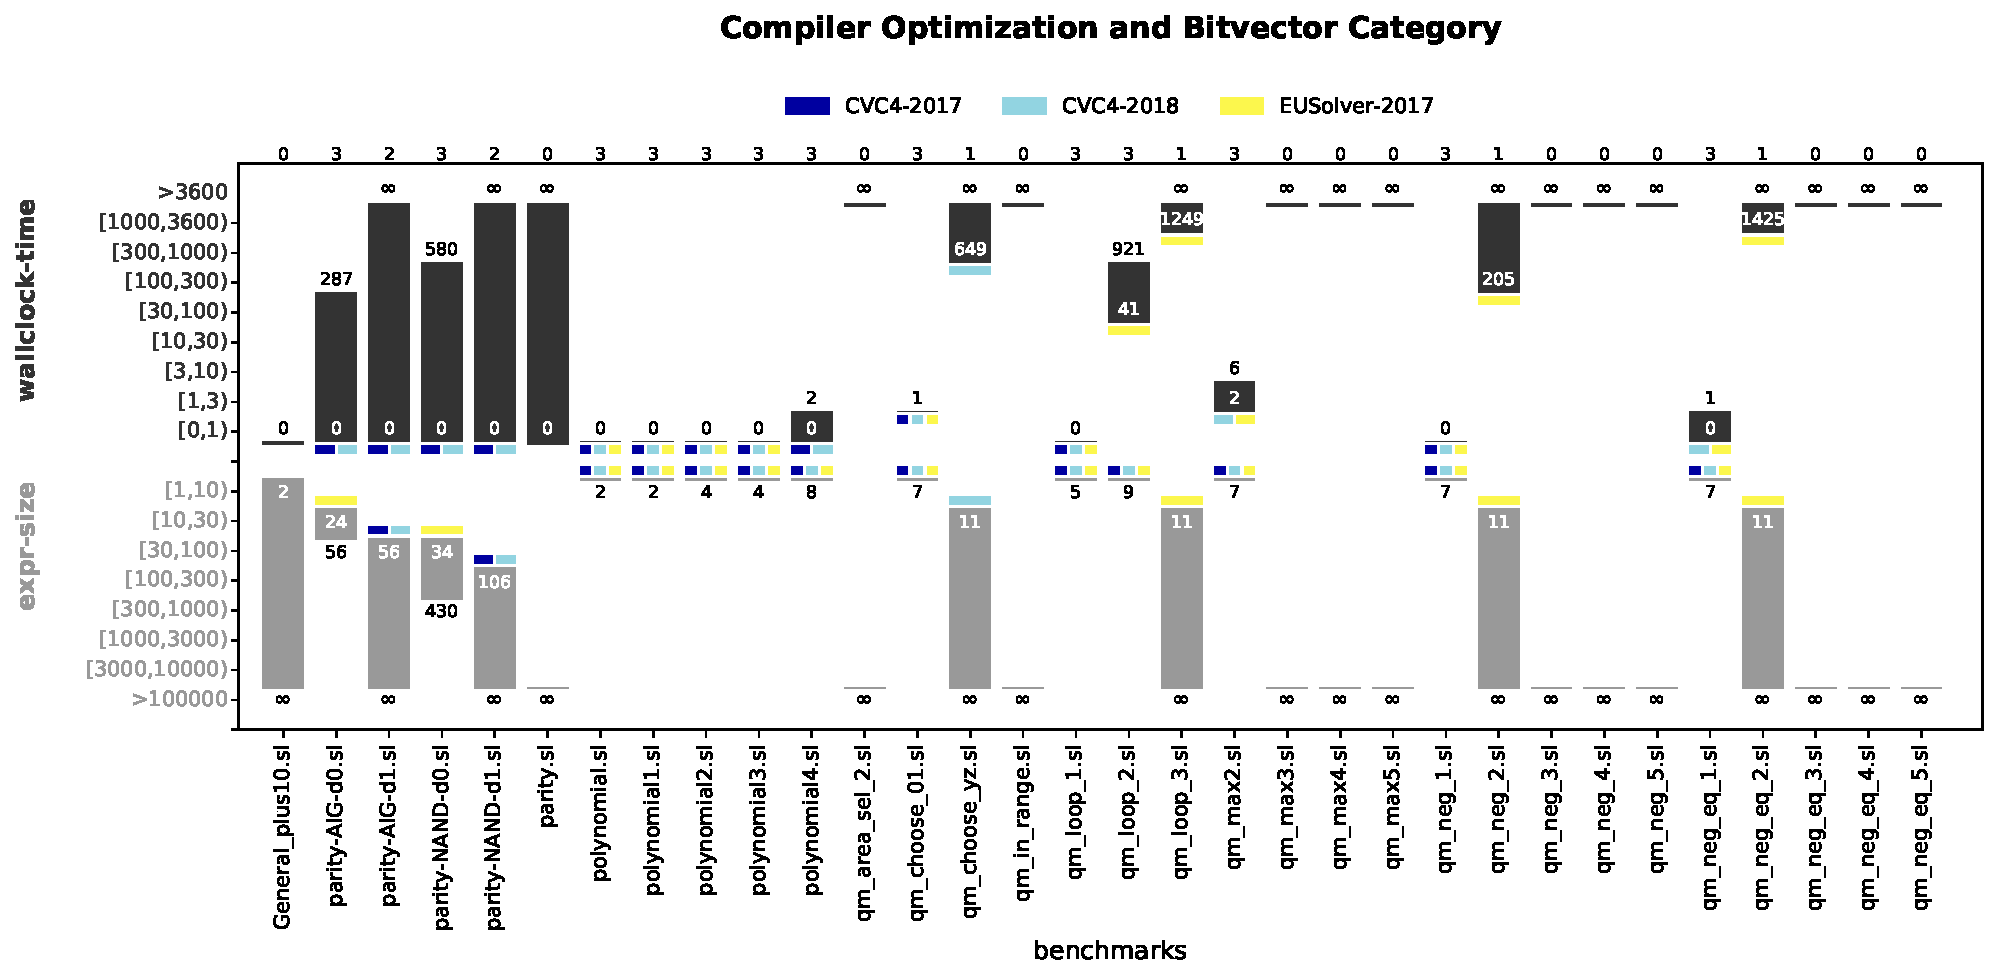
\includegraphics[width=10in]{figures/General1.pdf} \\[3cm]
				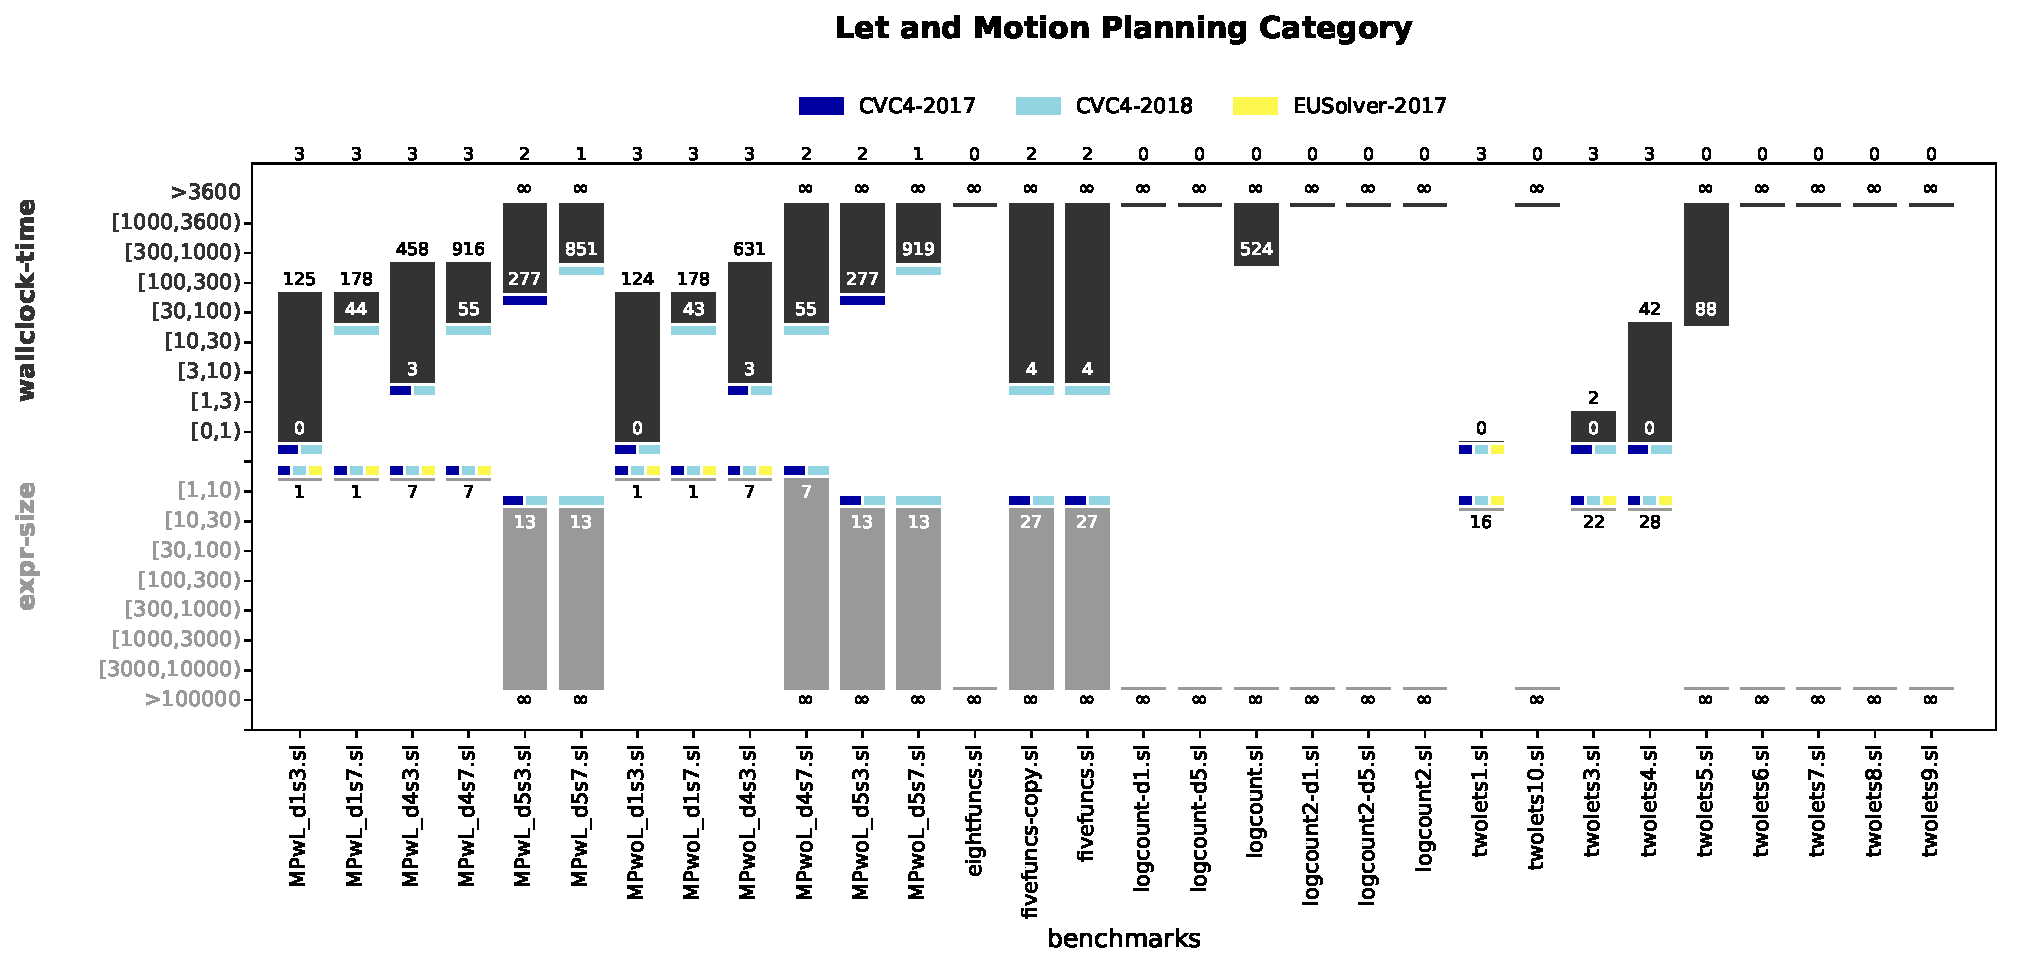
\includegraphics[width=10in]{figures/General2.pdf}
			\end{tabular}
	}}
	\caption{Evaluation of compiler optimizations, bitvectors, let and motion planning,
			 and program repair categories of the General track.}
	\label{fig:let-mot-plan}
\end{figure*}

\begin{figure*}
	\noindent\makebox[\textwidth]{
		\scalebox{0.625}{
			\begin{tabular}{c}
				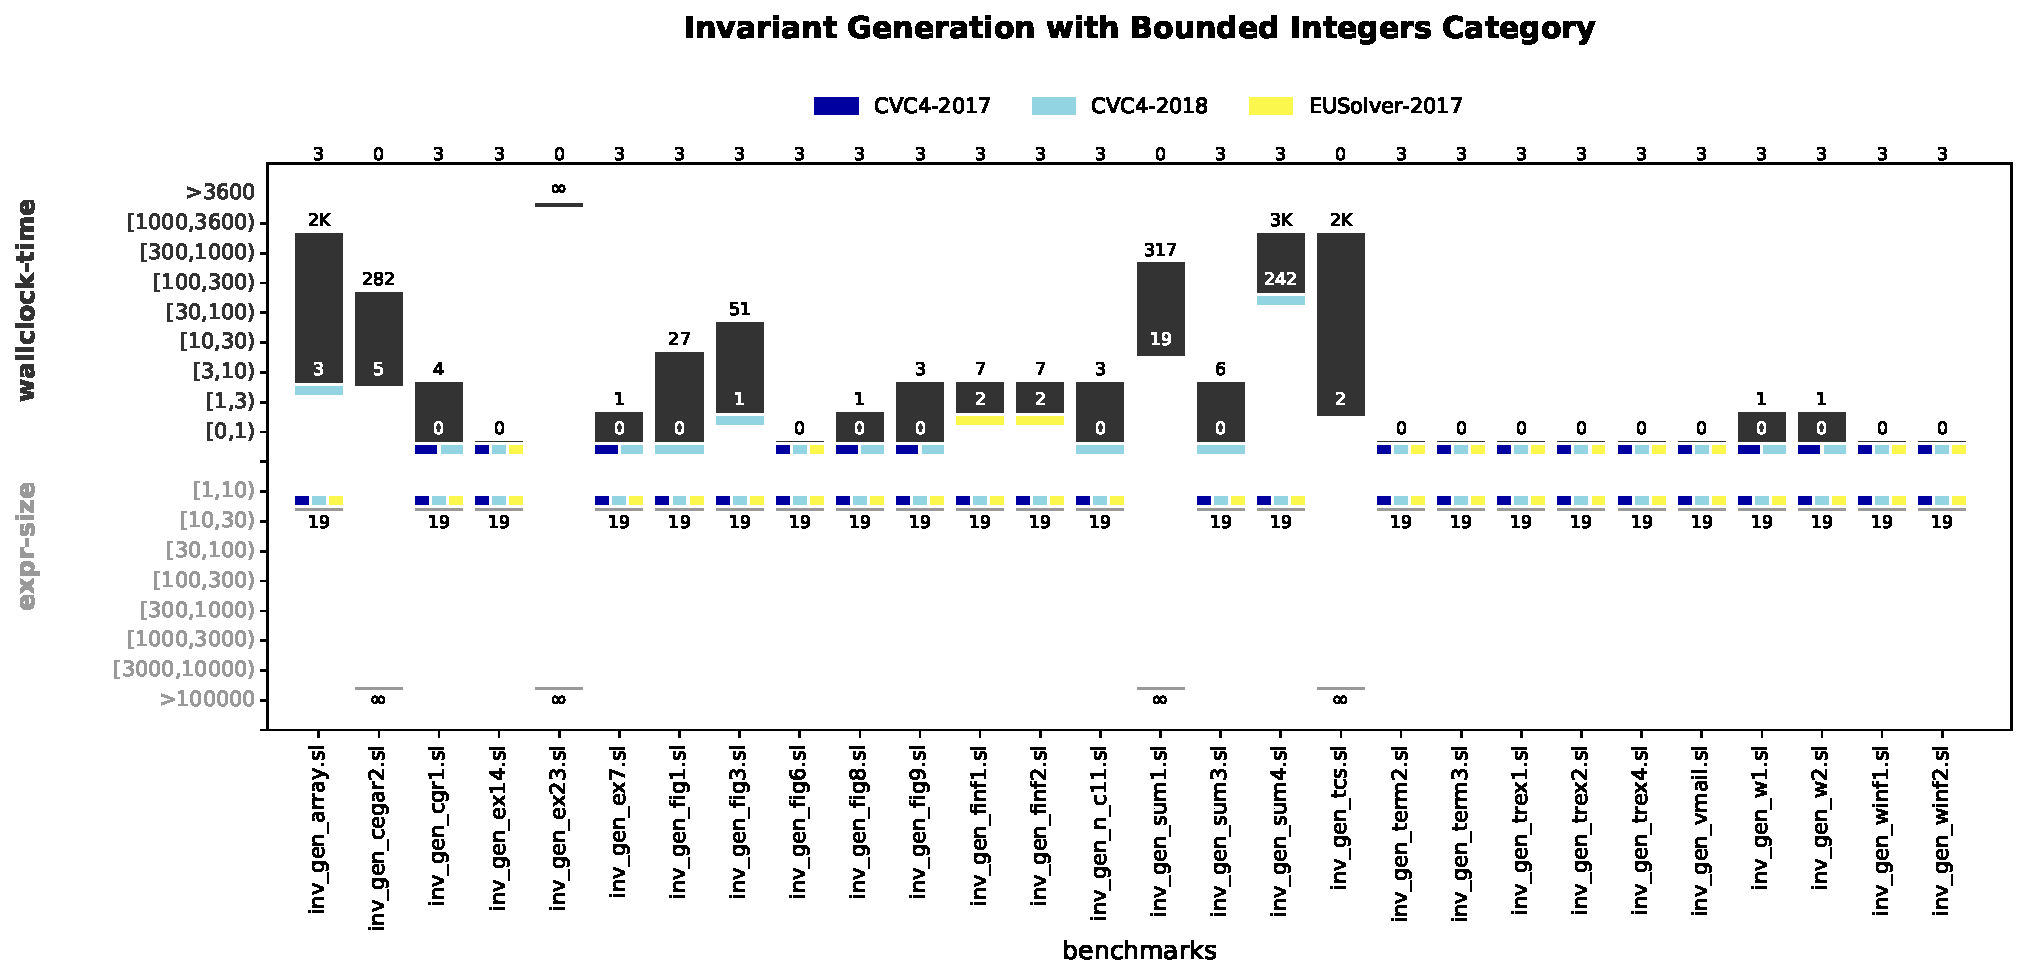
\includegraphics[width=10in]{figures/General3.pdf} \\[3cm]
				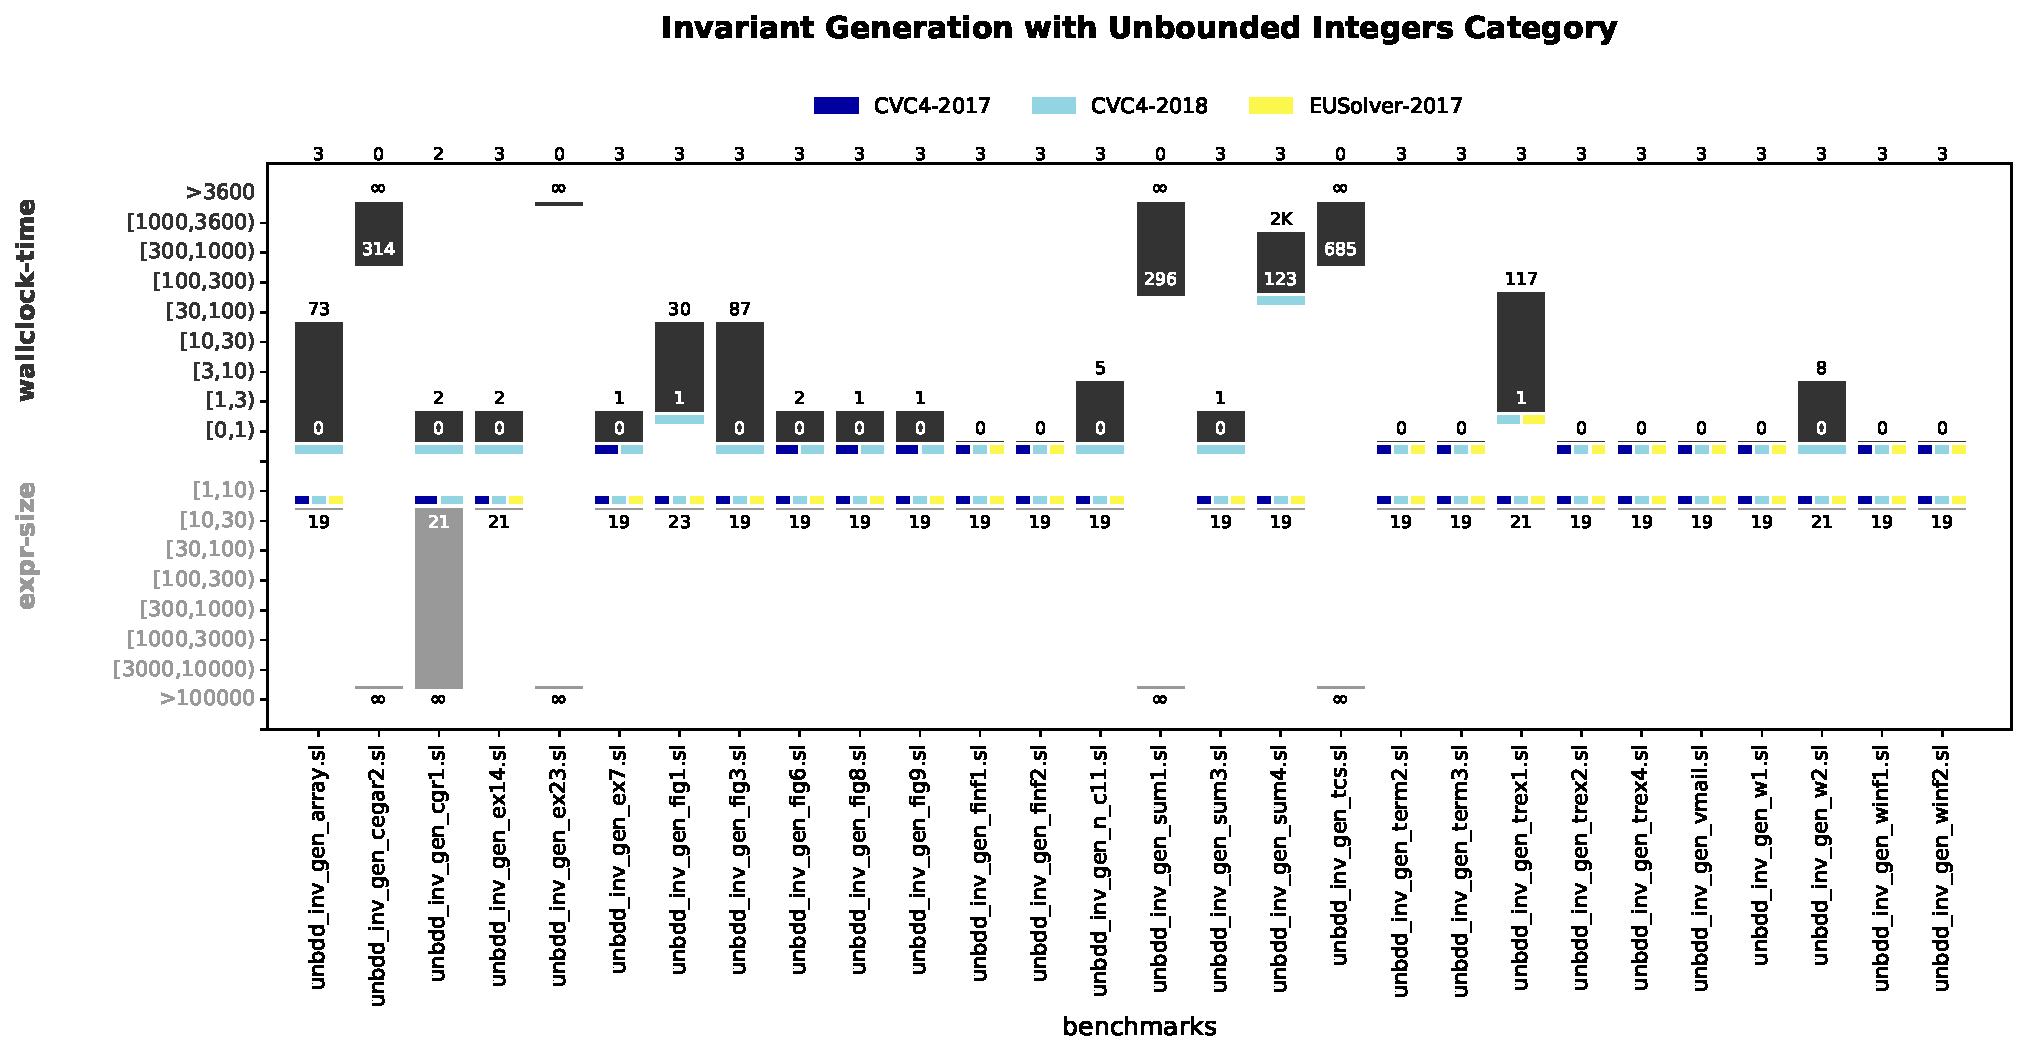
\includegraphics[width=10in]{figures/General4.pdf} 
			\end{tabular}
	}}
	\caption{Evaluation of invariant generation categories of the General track.}
	\label{fig:inv-results}
\end{figure*}

\begin{figure*}
	\noindent\makebox[\textwidth]{
		\scalebox{0.625}{
			\begin{tabular}{c}
				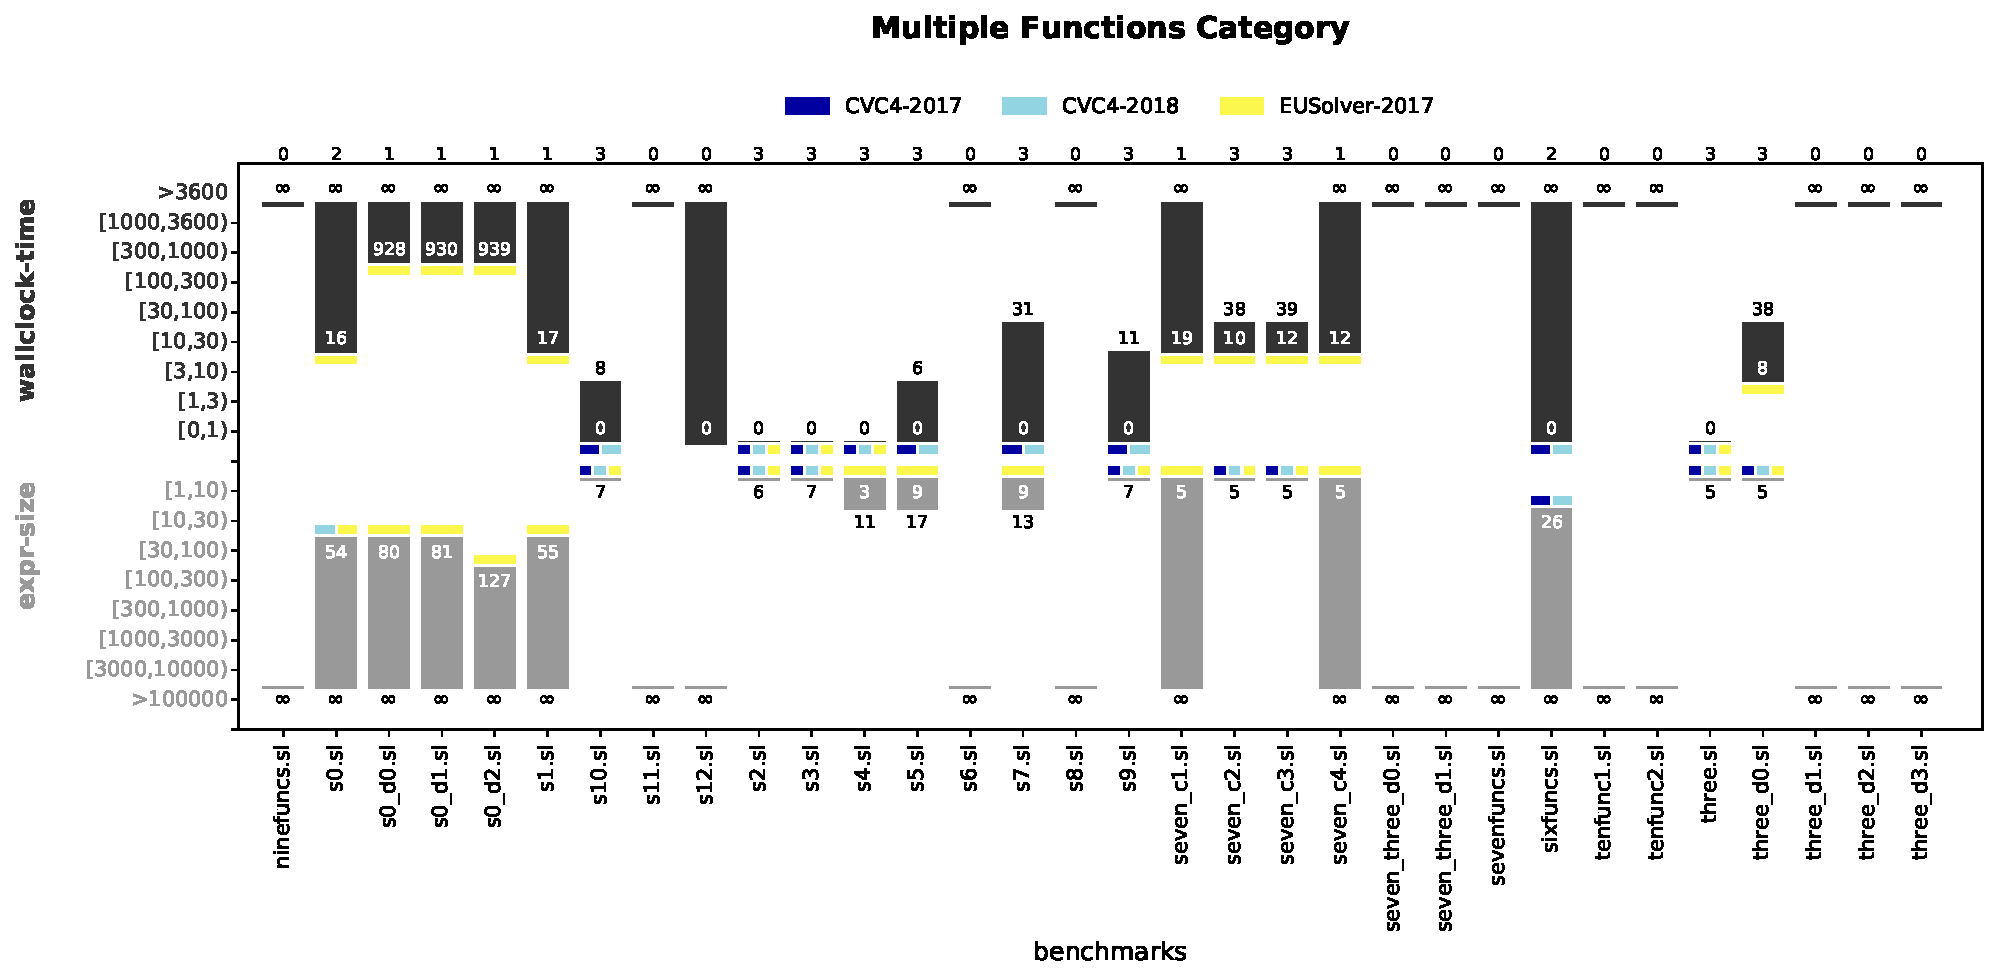
\includegraphics[width=10in]{figures/General5.pdf} \\[3cm]
				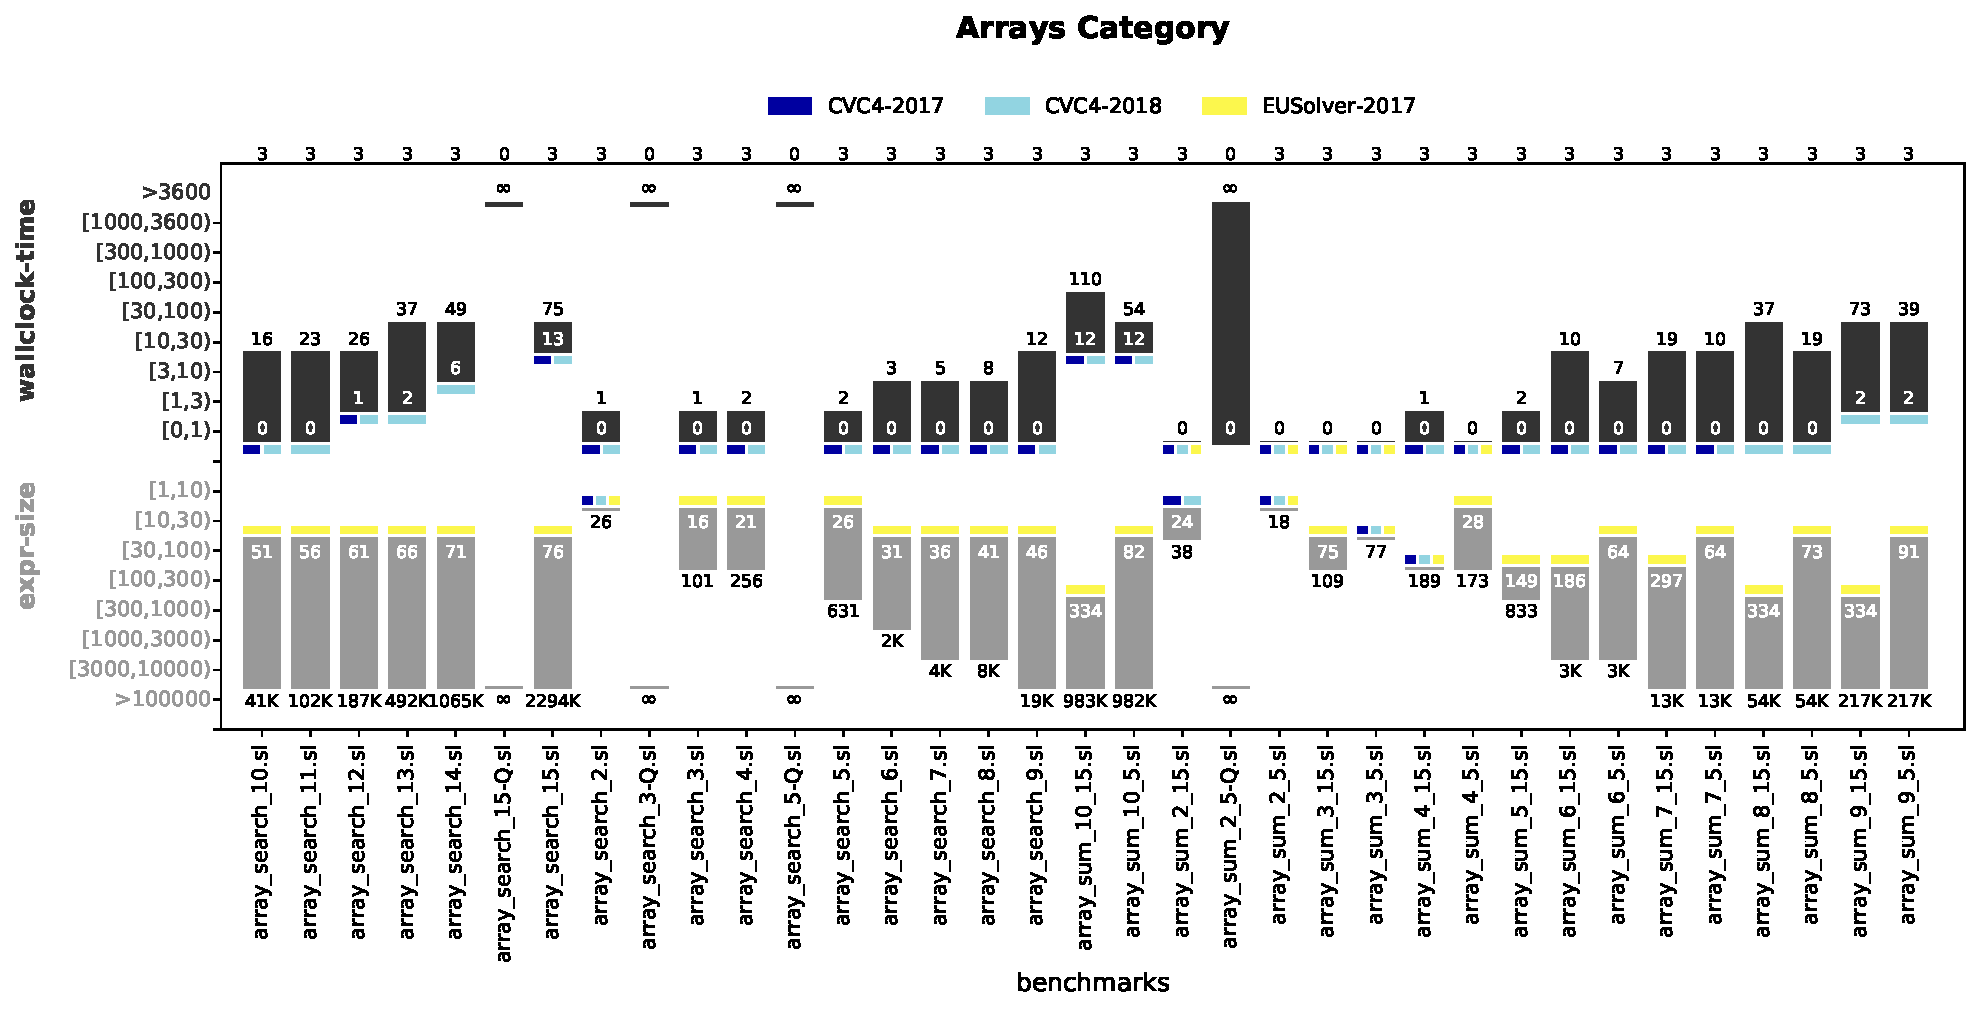
\includegraphics[width=10in]{figures/General6.pdf} 
			\end{tabular}
	}}
	\caption{Evaluation of multiple functions and arrays categories of the General track.}
	\label{fig:mult-func-arr}
\end{figure*}

\begin{figure*}
	\noindent\makebox[\textwidth]{
		\scalebox{0.6}{
			\begin{tabular}{c}
				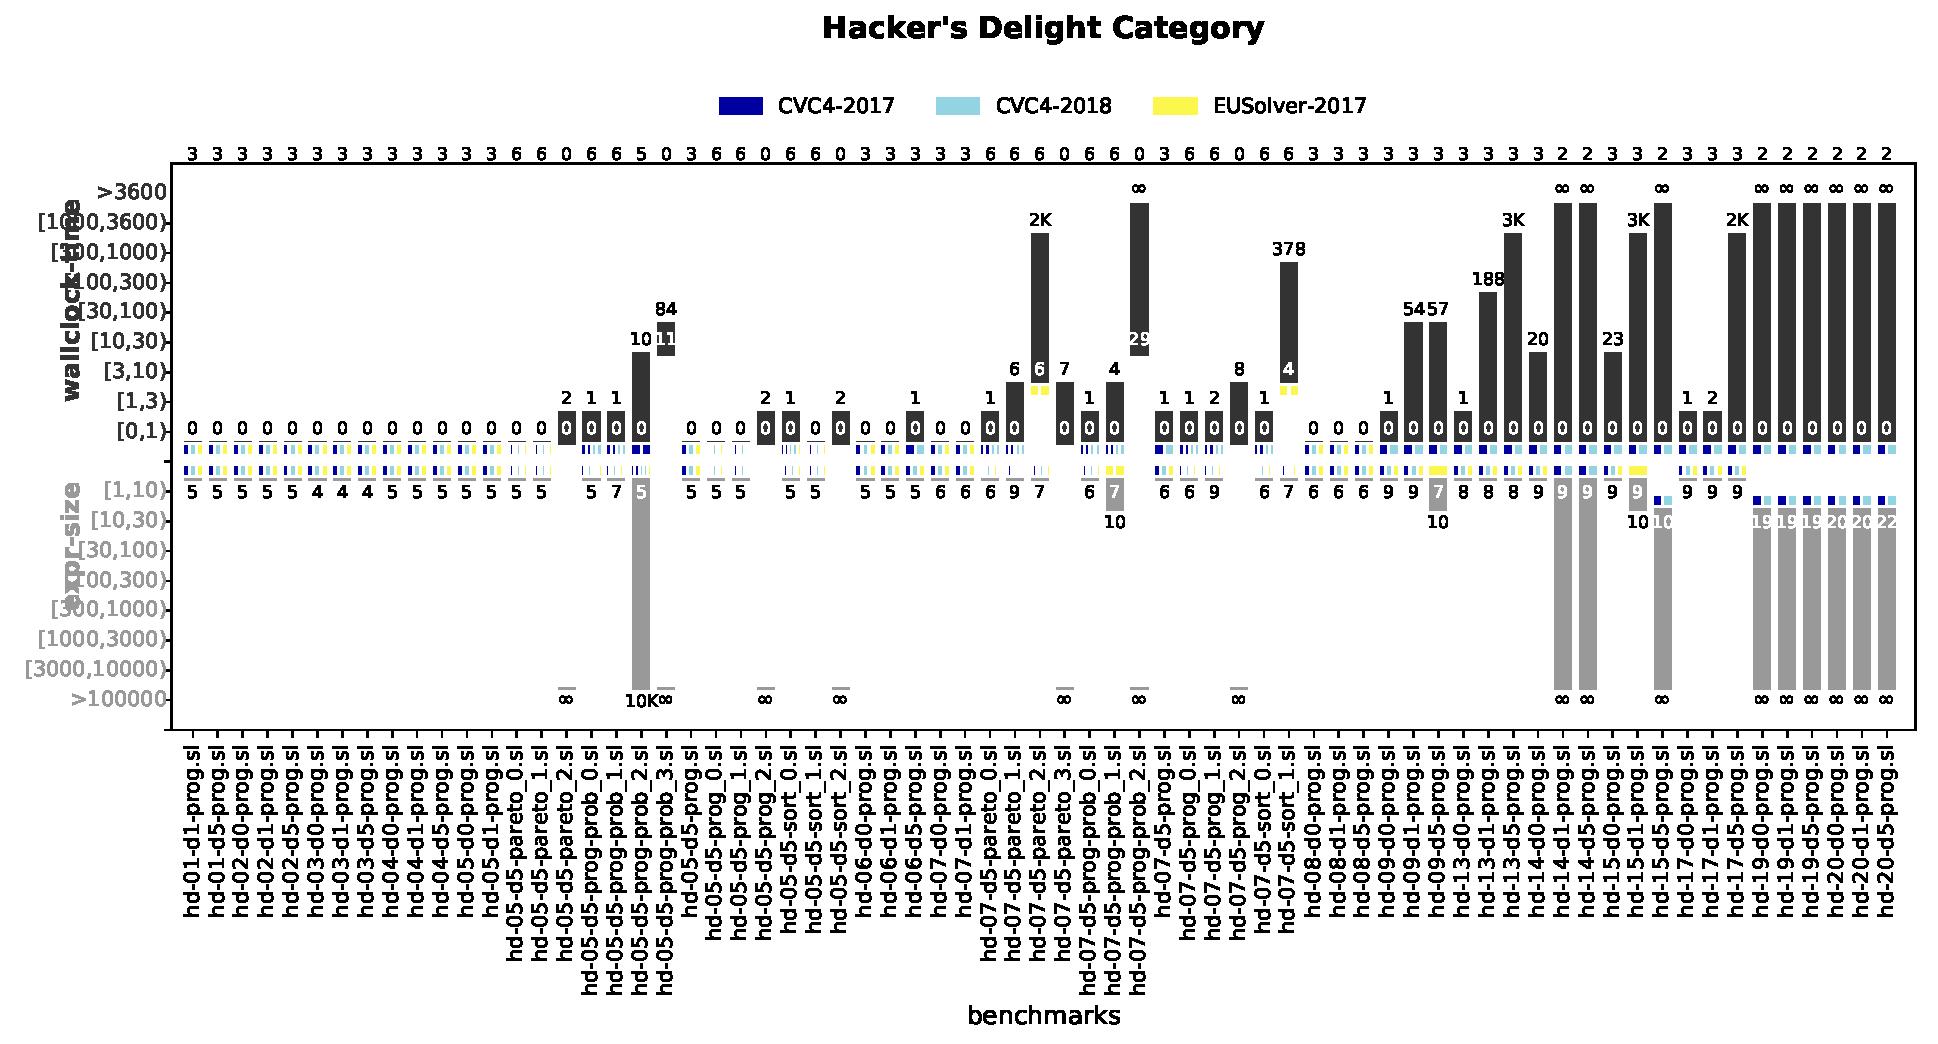
\includegraphics[width=10in]{figures/General7.pdf} \\[3cm]
				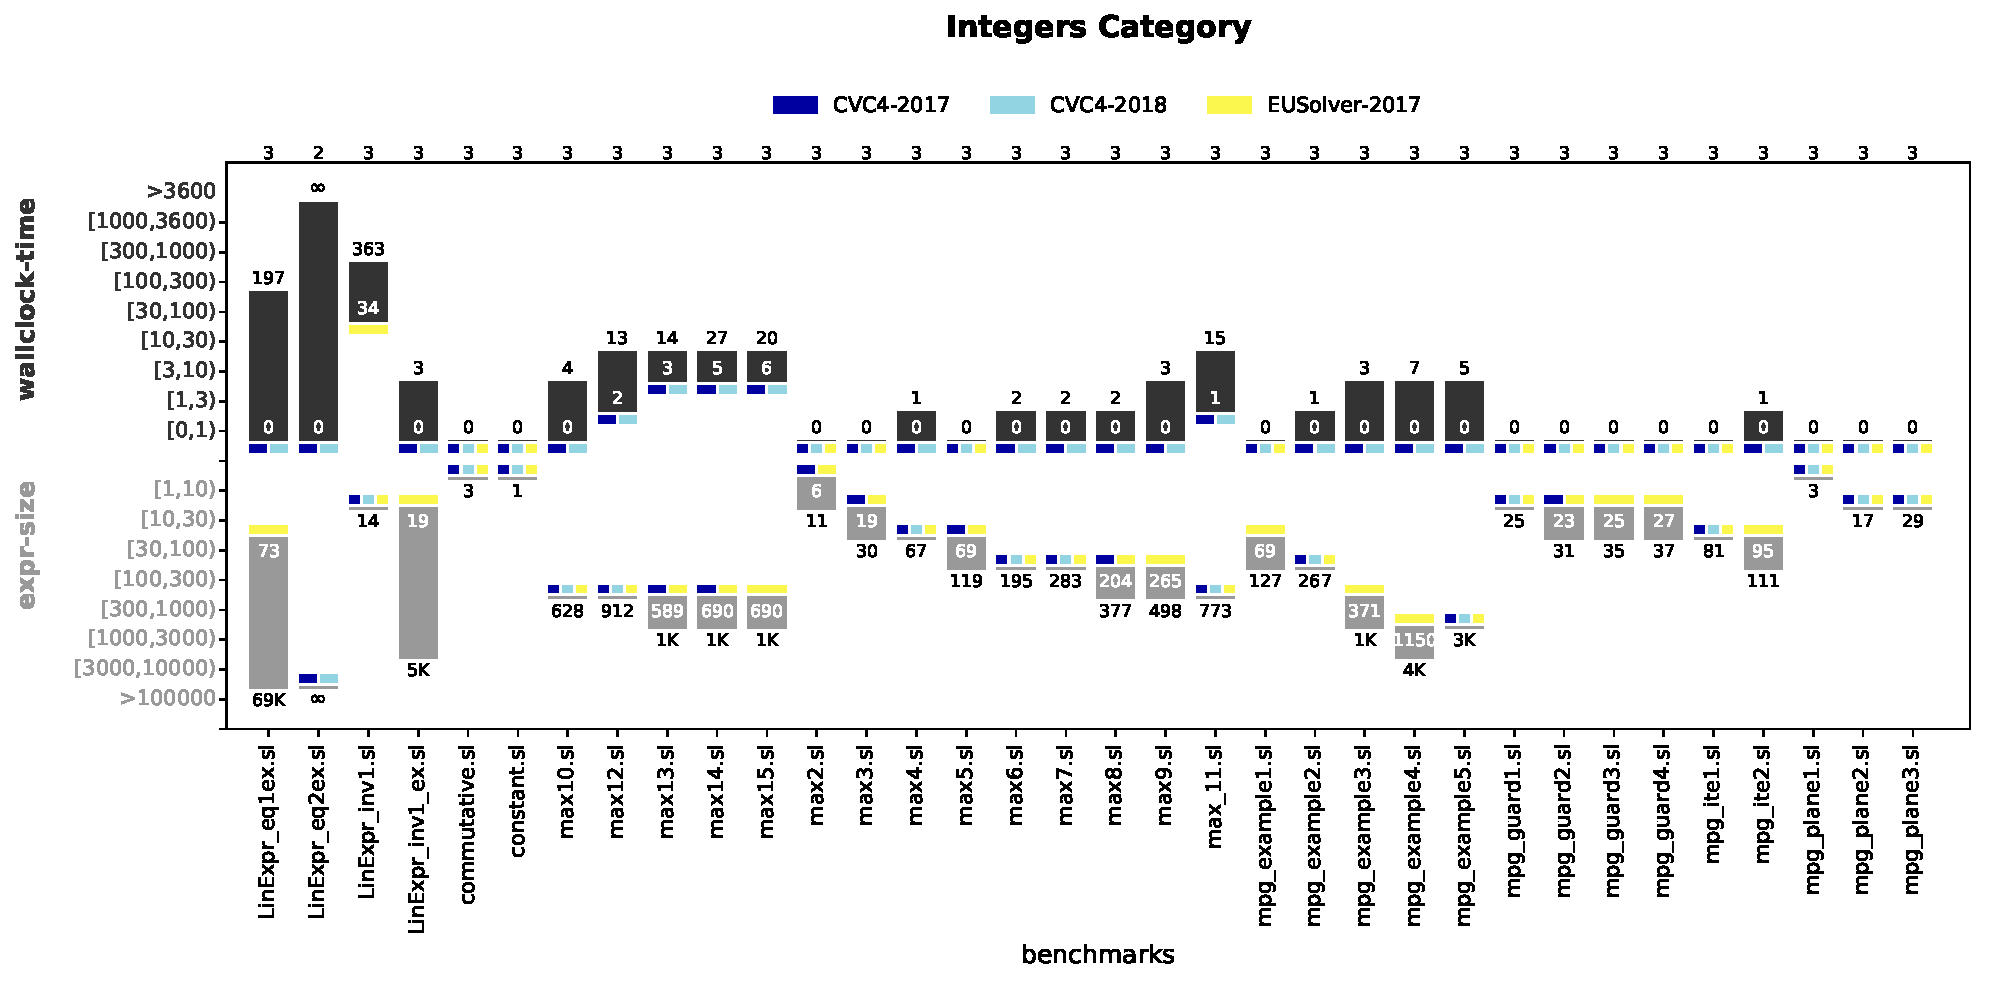
\includegraphics[width=10in]{figures/General8.pdf} 
			\end{tabular}
	}}
	\caption{Evaluation of hacker's delight and integers categories of the General track.}
	\label{fig:hd-int}
\end{figure*}

\begin{figure*}
	\noindent\makebox[\textwidth]{
		\scalebox{0.625}{
			\begin{tabular}{c}
				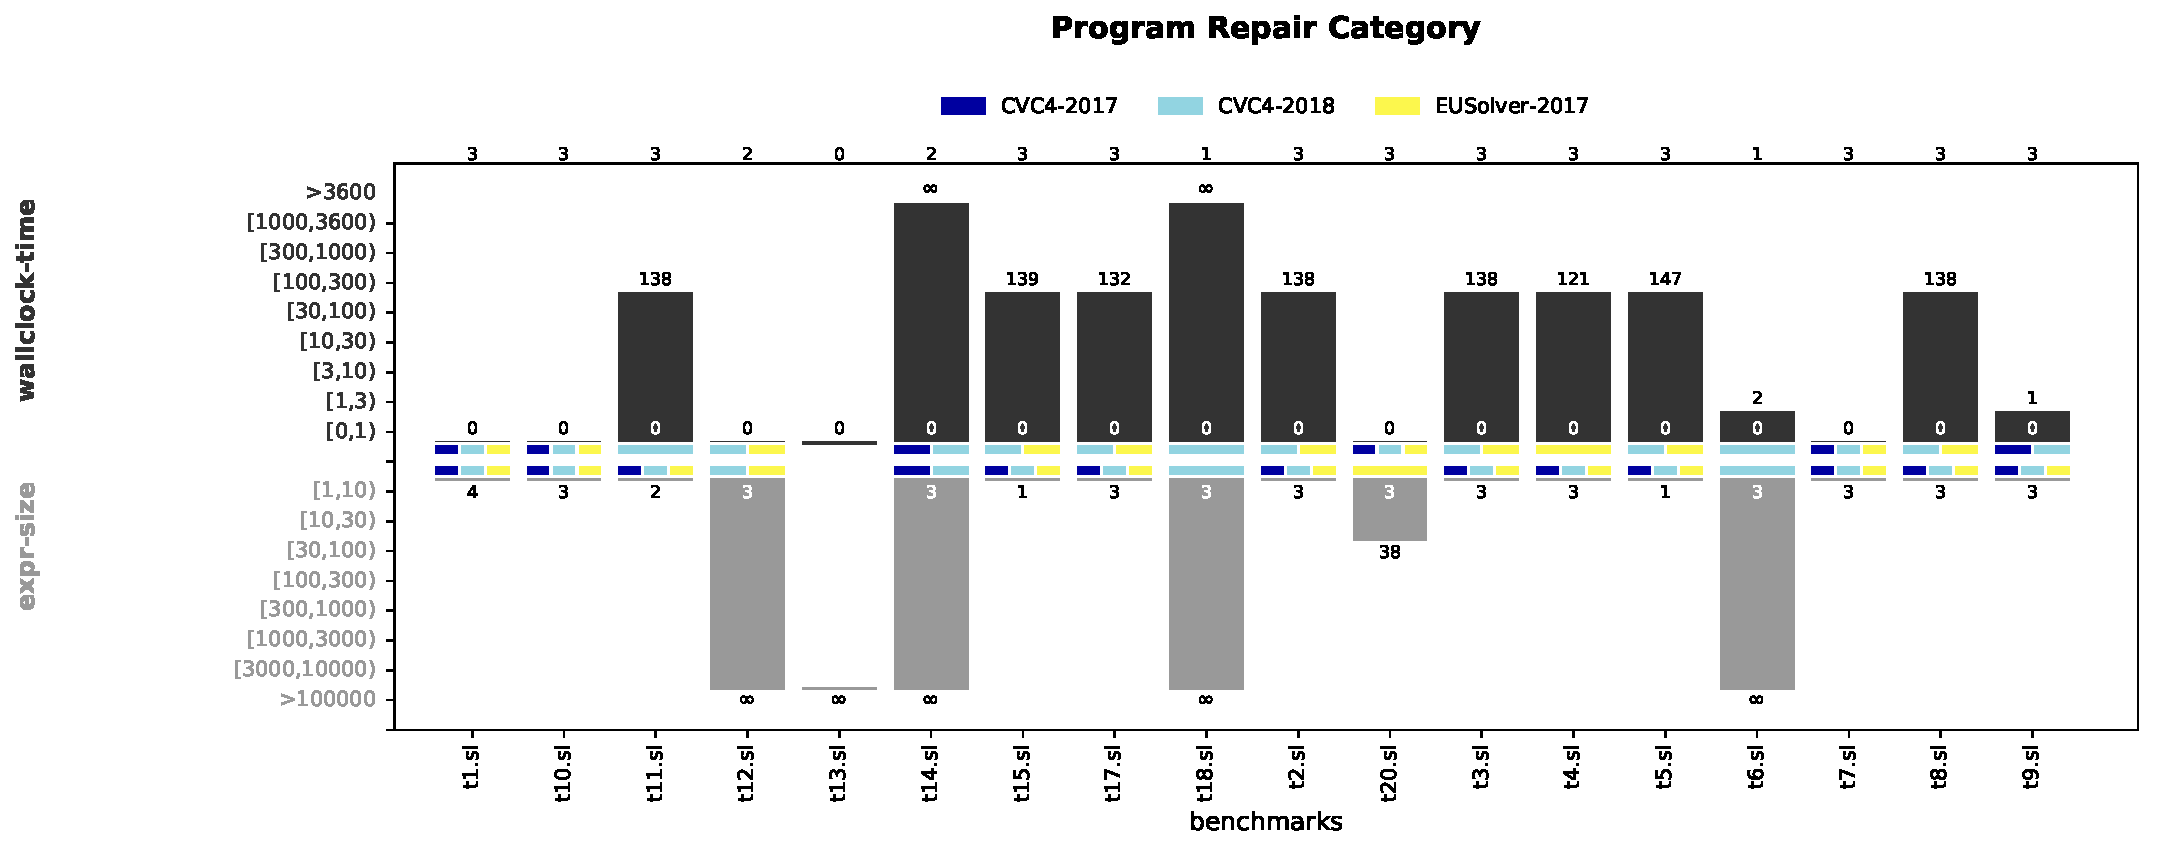
\includegraphics[width=10in]{figures/General9.pdf} \\[3cm]
				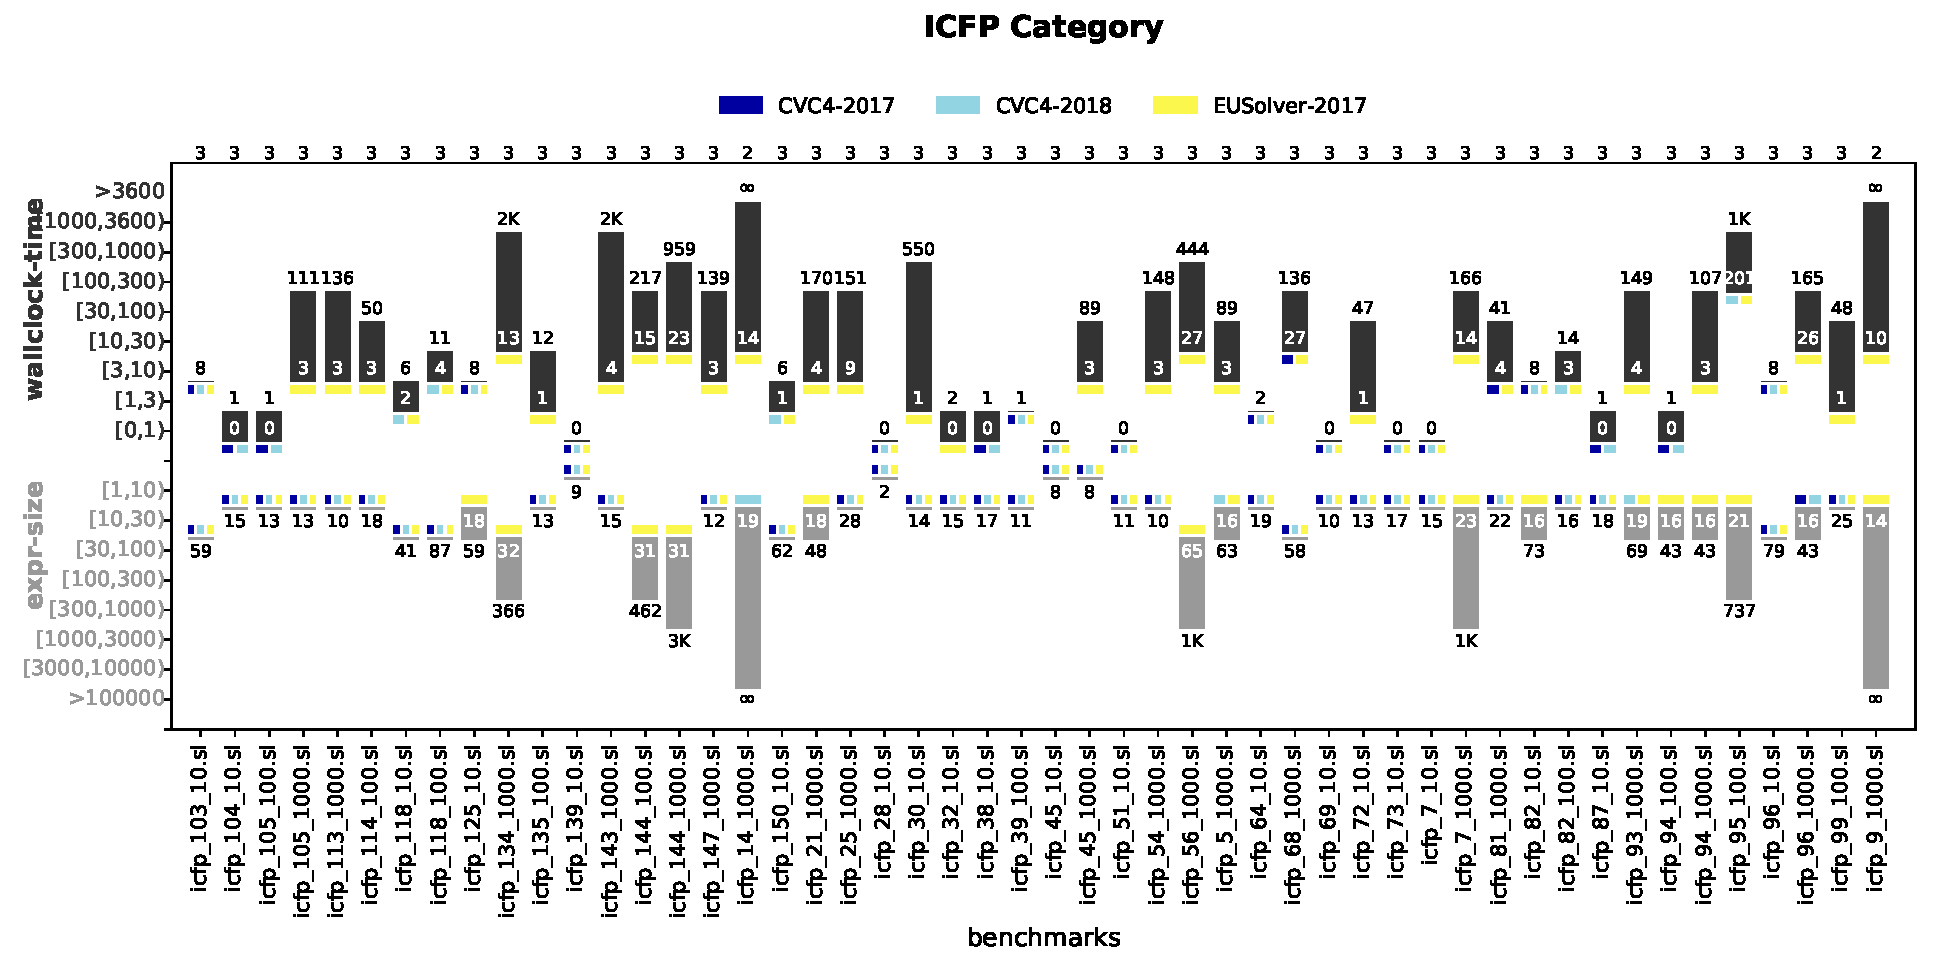
\includegraphics[width=10in]{figures/General10.pdf}
			\end{tabular}
	}}
	\caption{Evaluation of program repair and ICFP categories of the General track.}
	\label{fig:prog-rep-icfp}
\end{figure*}

\begin{figure*}
	\noindent\makebox[\textwidth]{
		\scalebox{0.625}{
			\begin{tabular}{c}
				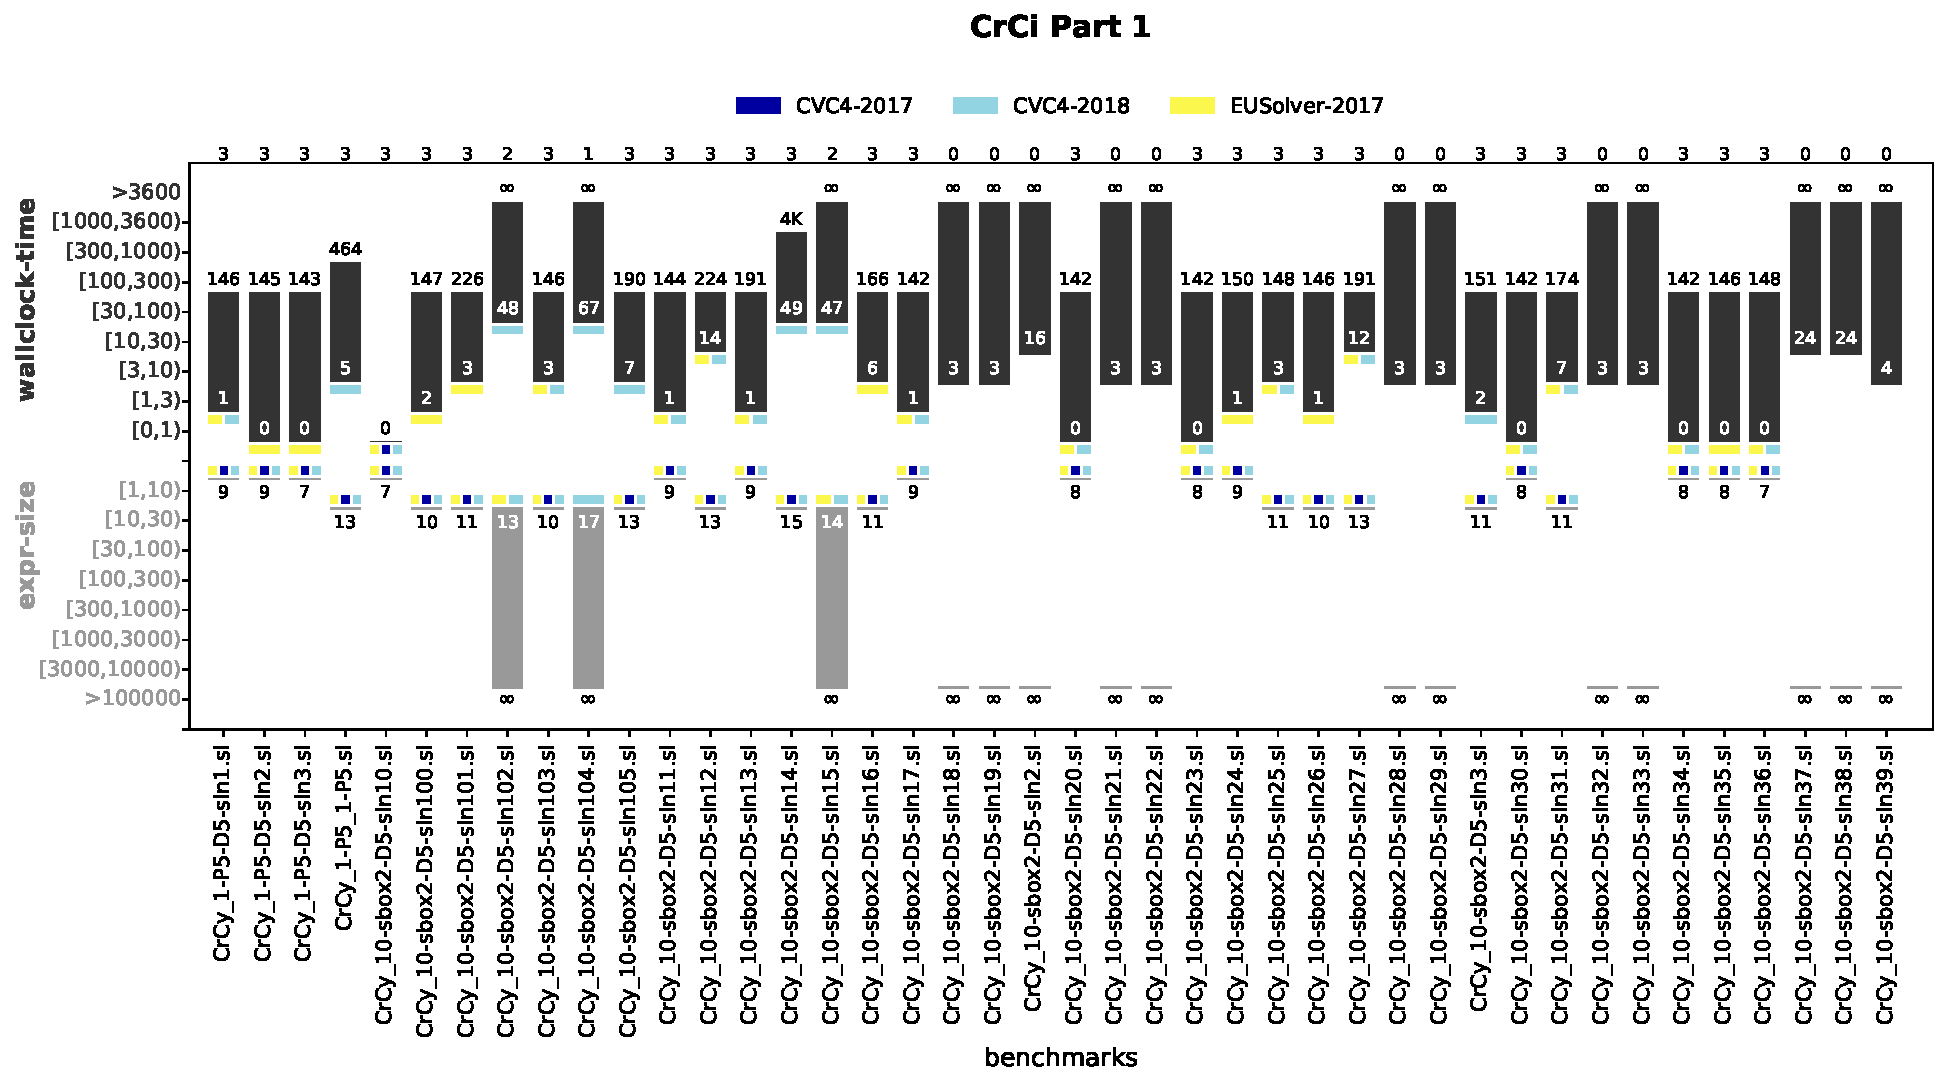
\includegraphics[width=10in]{figures/CrCi1.pdf} \\[3cm]
				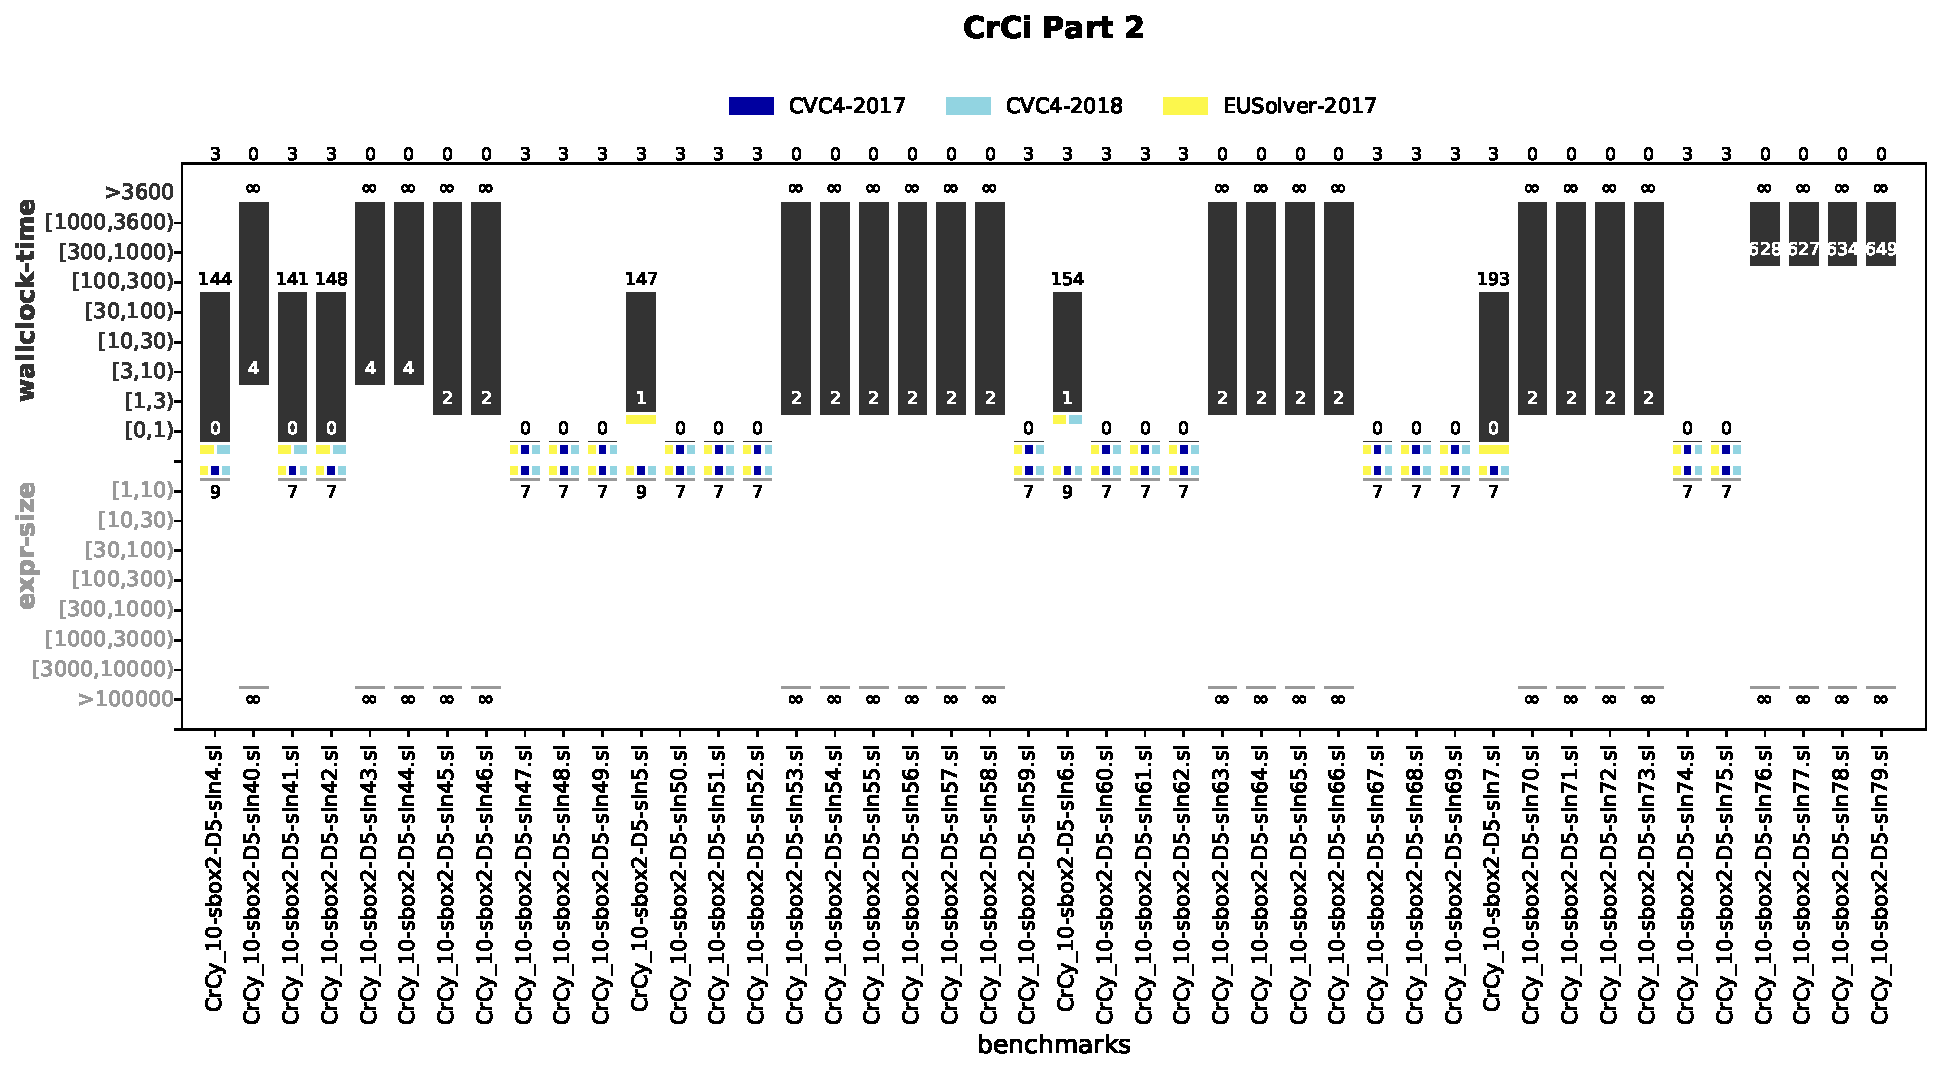
\includegraphics[width=10in]{figures/CrCi2.pdf}
			\end{tabular}
	}}
	\caption{Evaluation of crypto circuits category of the General track (Parts 1 \& 2).}
	\label{fig:crci-1}
\end{figure*}

\begin{figure*}
	\noindent\makebox[\textwidth]{
		\scalebox{0.625}{
			\begin{tabular}{c}
				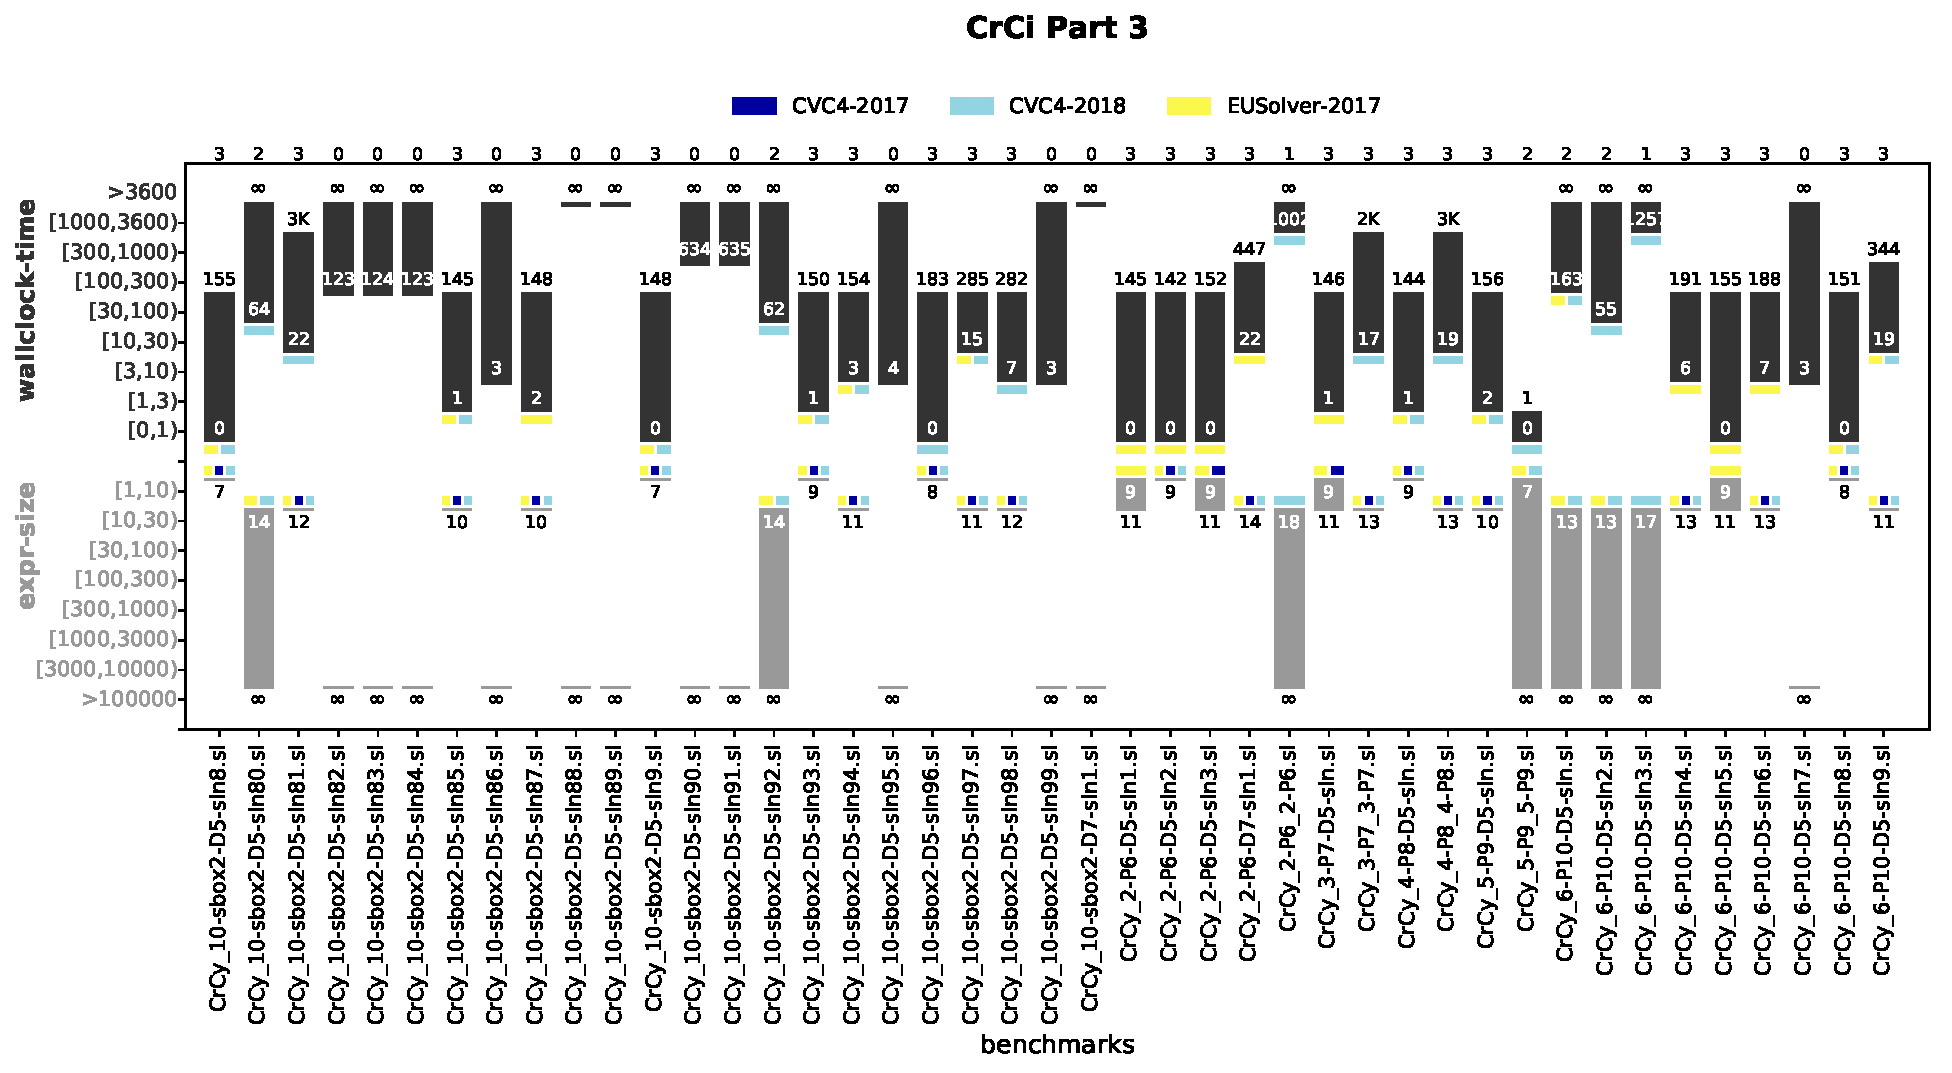
\includegraphics[width=10in]{figures/CrCi3.pdf} \\[3cm]
				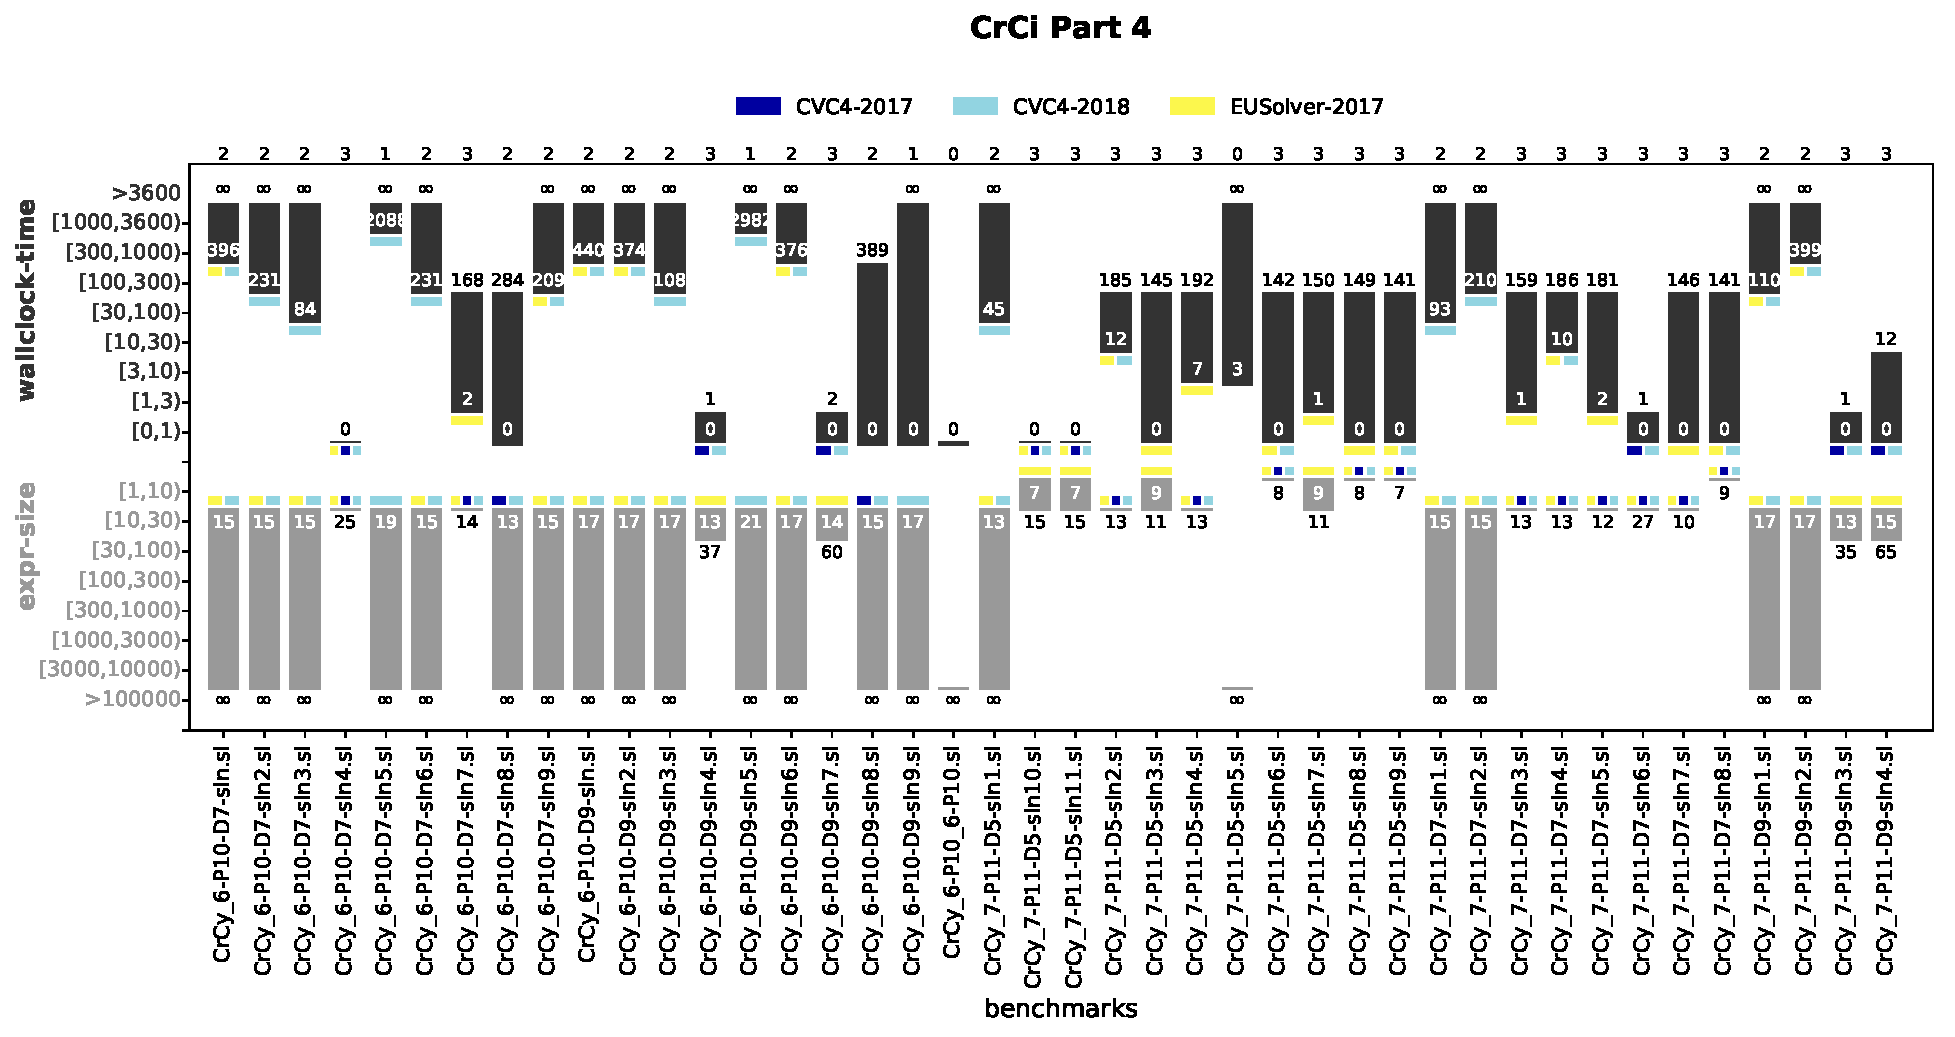
\includegraphics[width=10in]{figures/CrCi4.pdf}
			\end{tabular}
	}}
	\caption{Evaluation of crypto circuits category of the General track (Parts 3 \& 4).}
	\label{fig:crci-2}
\end{figure*}
	
\begin{figure*}
	\noindent\makebox[\textwidth]{
		\scalebox{0.625}{
			\begin{tabular}{c}
				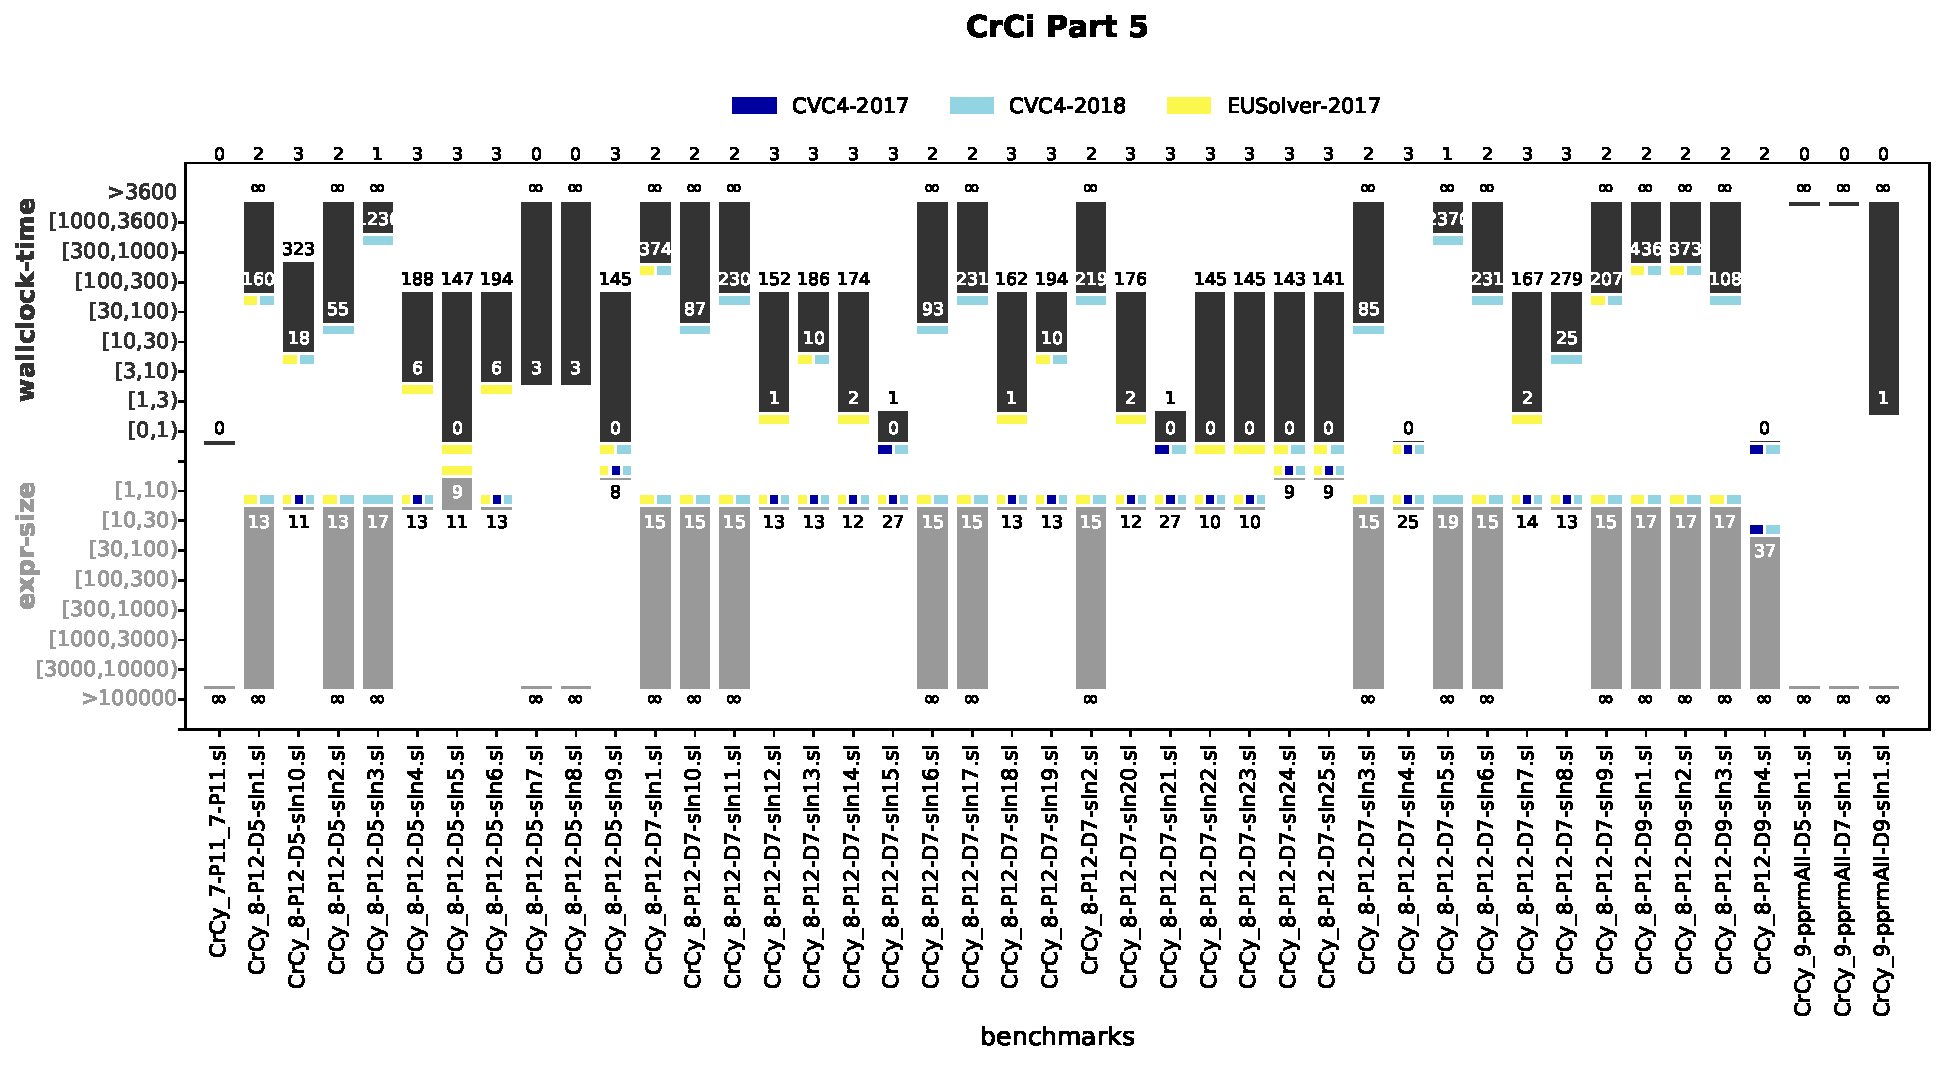
\includegraphics[width=10in]{figures/CrCi5.pdf}
			\end{tabular}
	}}
	\caption{Evaluation of crypto circuits category of the General track (Part 5).}
	\label{fig:crci-5}
\end{figure*}
	

\begin{figure*}
	\noindent\makebox[\textwidth]{
		\scalebox{0.6}{
			\begin{tabular}{c}
				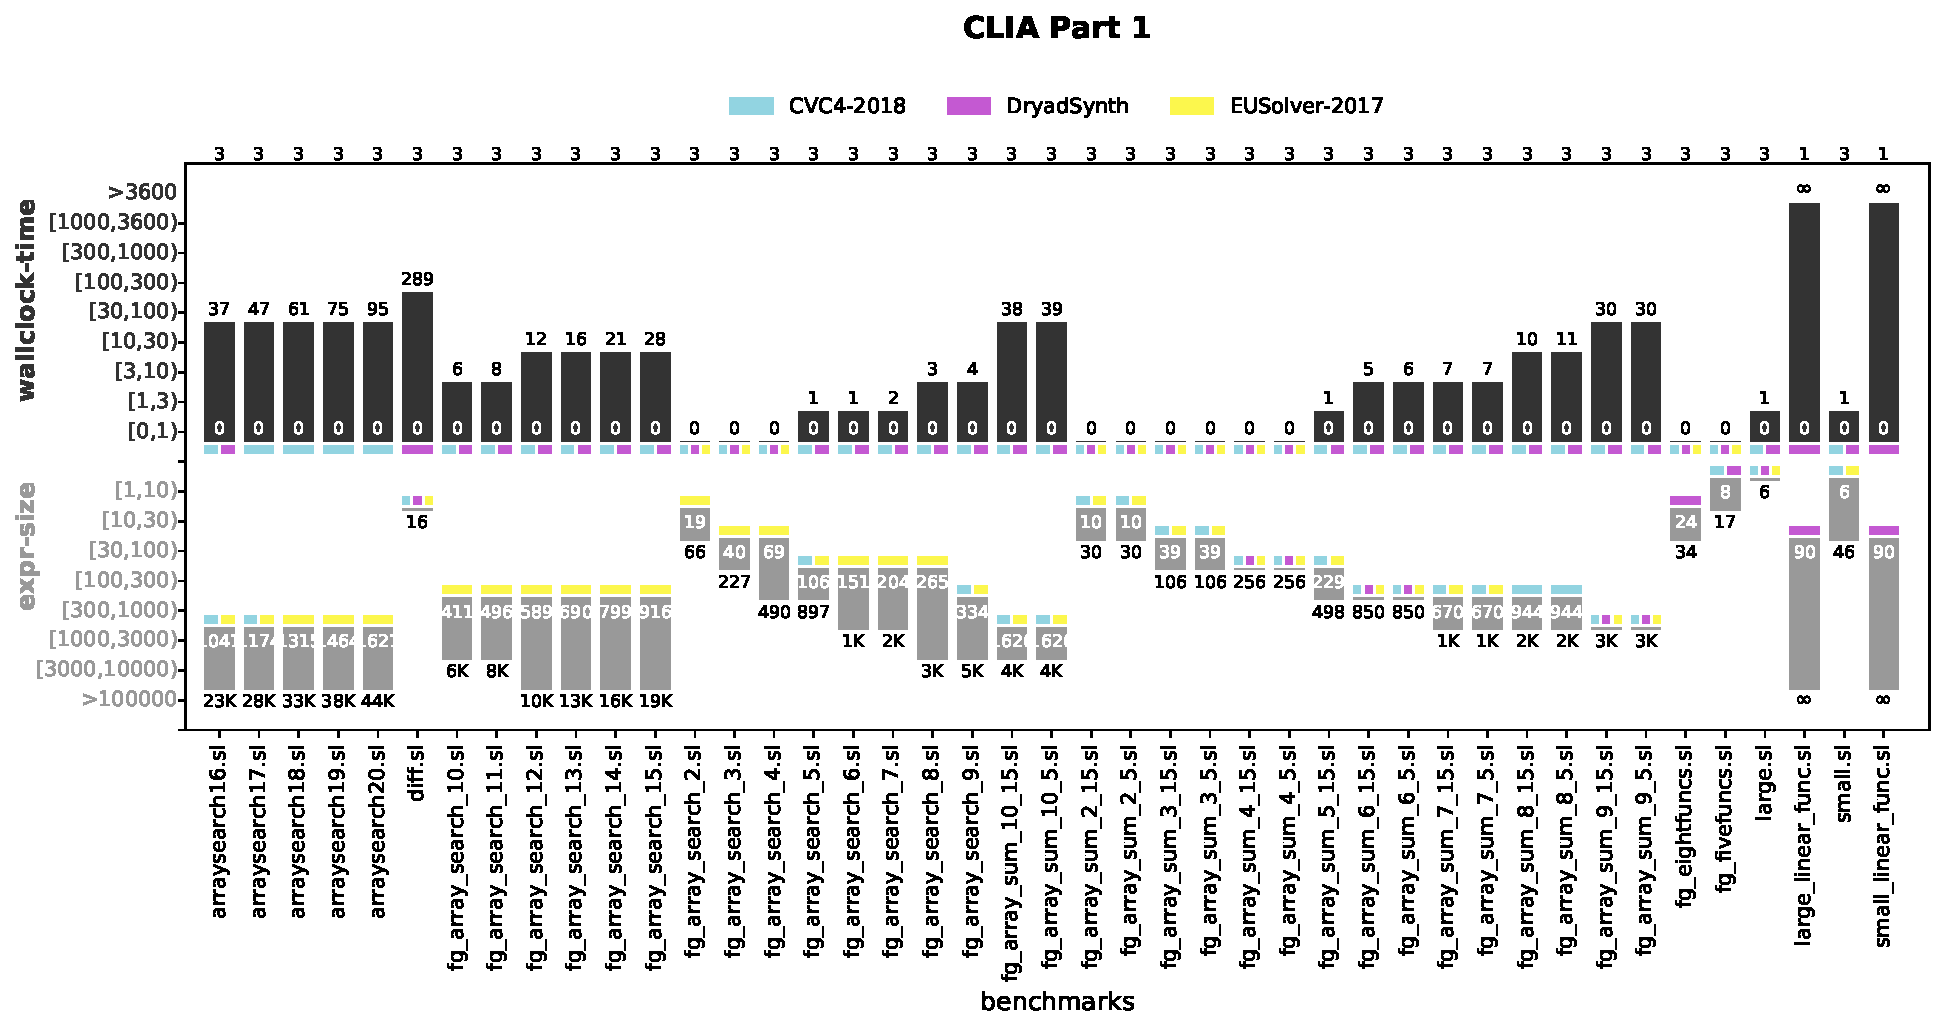
\includegraphics[width=10in]{figures/CLIA1.pdf} \\[3cm]
				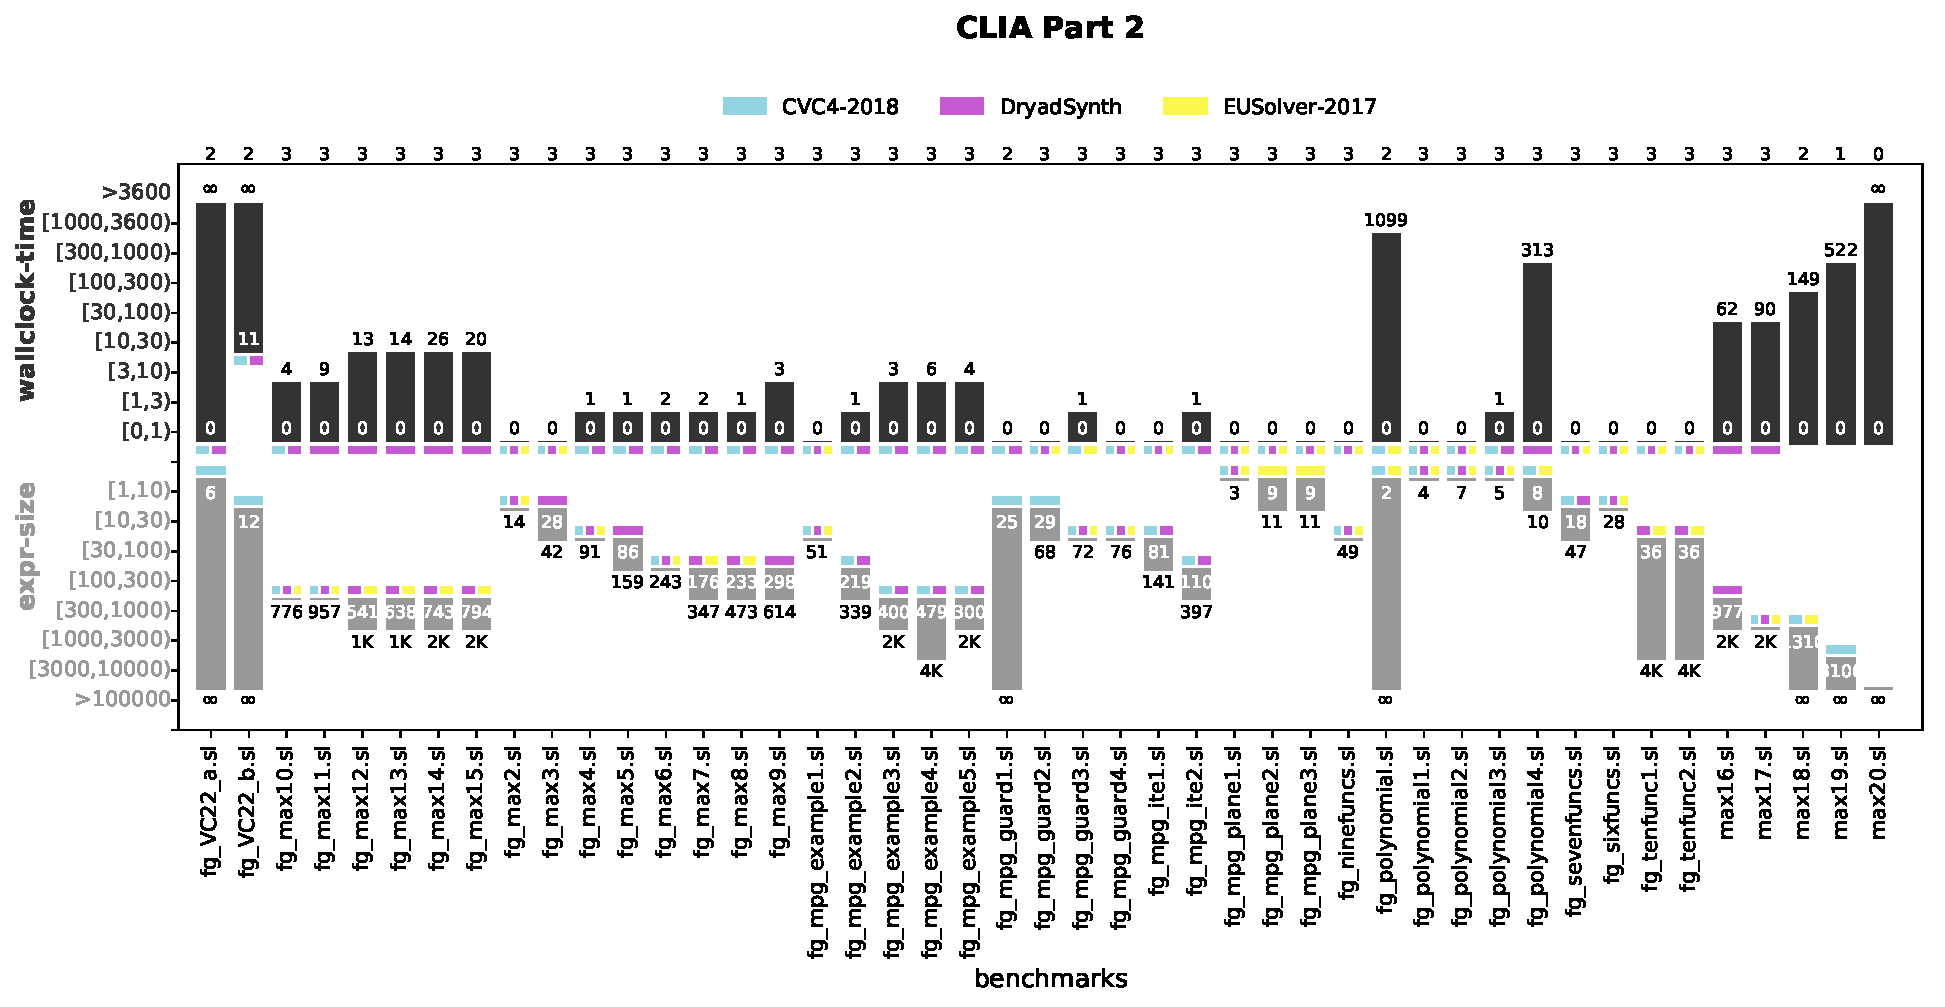
\includegraphics[width=10in]{figures/CLIA2.pdf} 
			\end{tabular}
	}}
	\caption{Evaluation of CLIA track benchmarks.}
	\label{fig:clia-results}
\end{figure*}



\begin{figure*}
	\noindent\makebox[\textwidth]{
		\scalebox{0.6}{
			\begin{tabular}{c}
				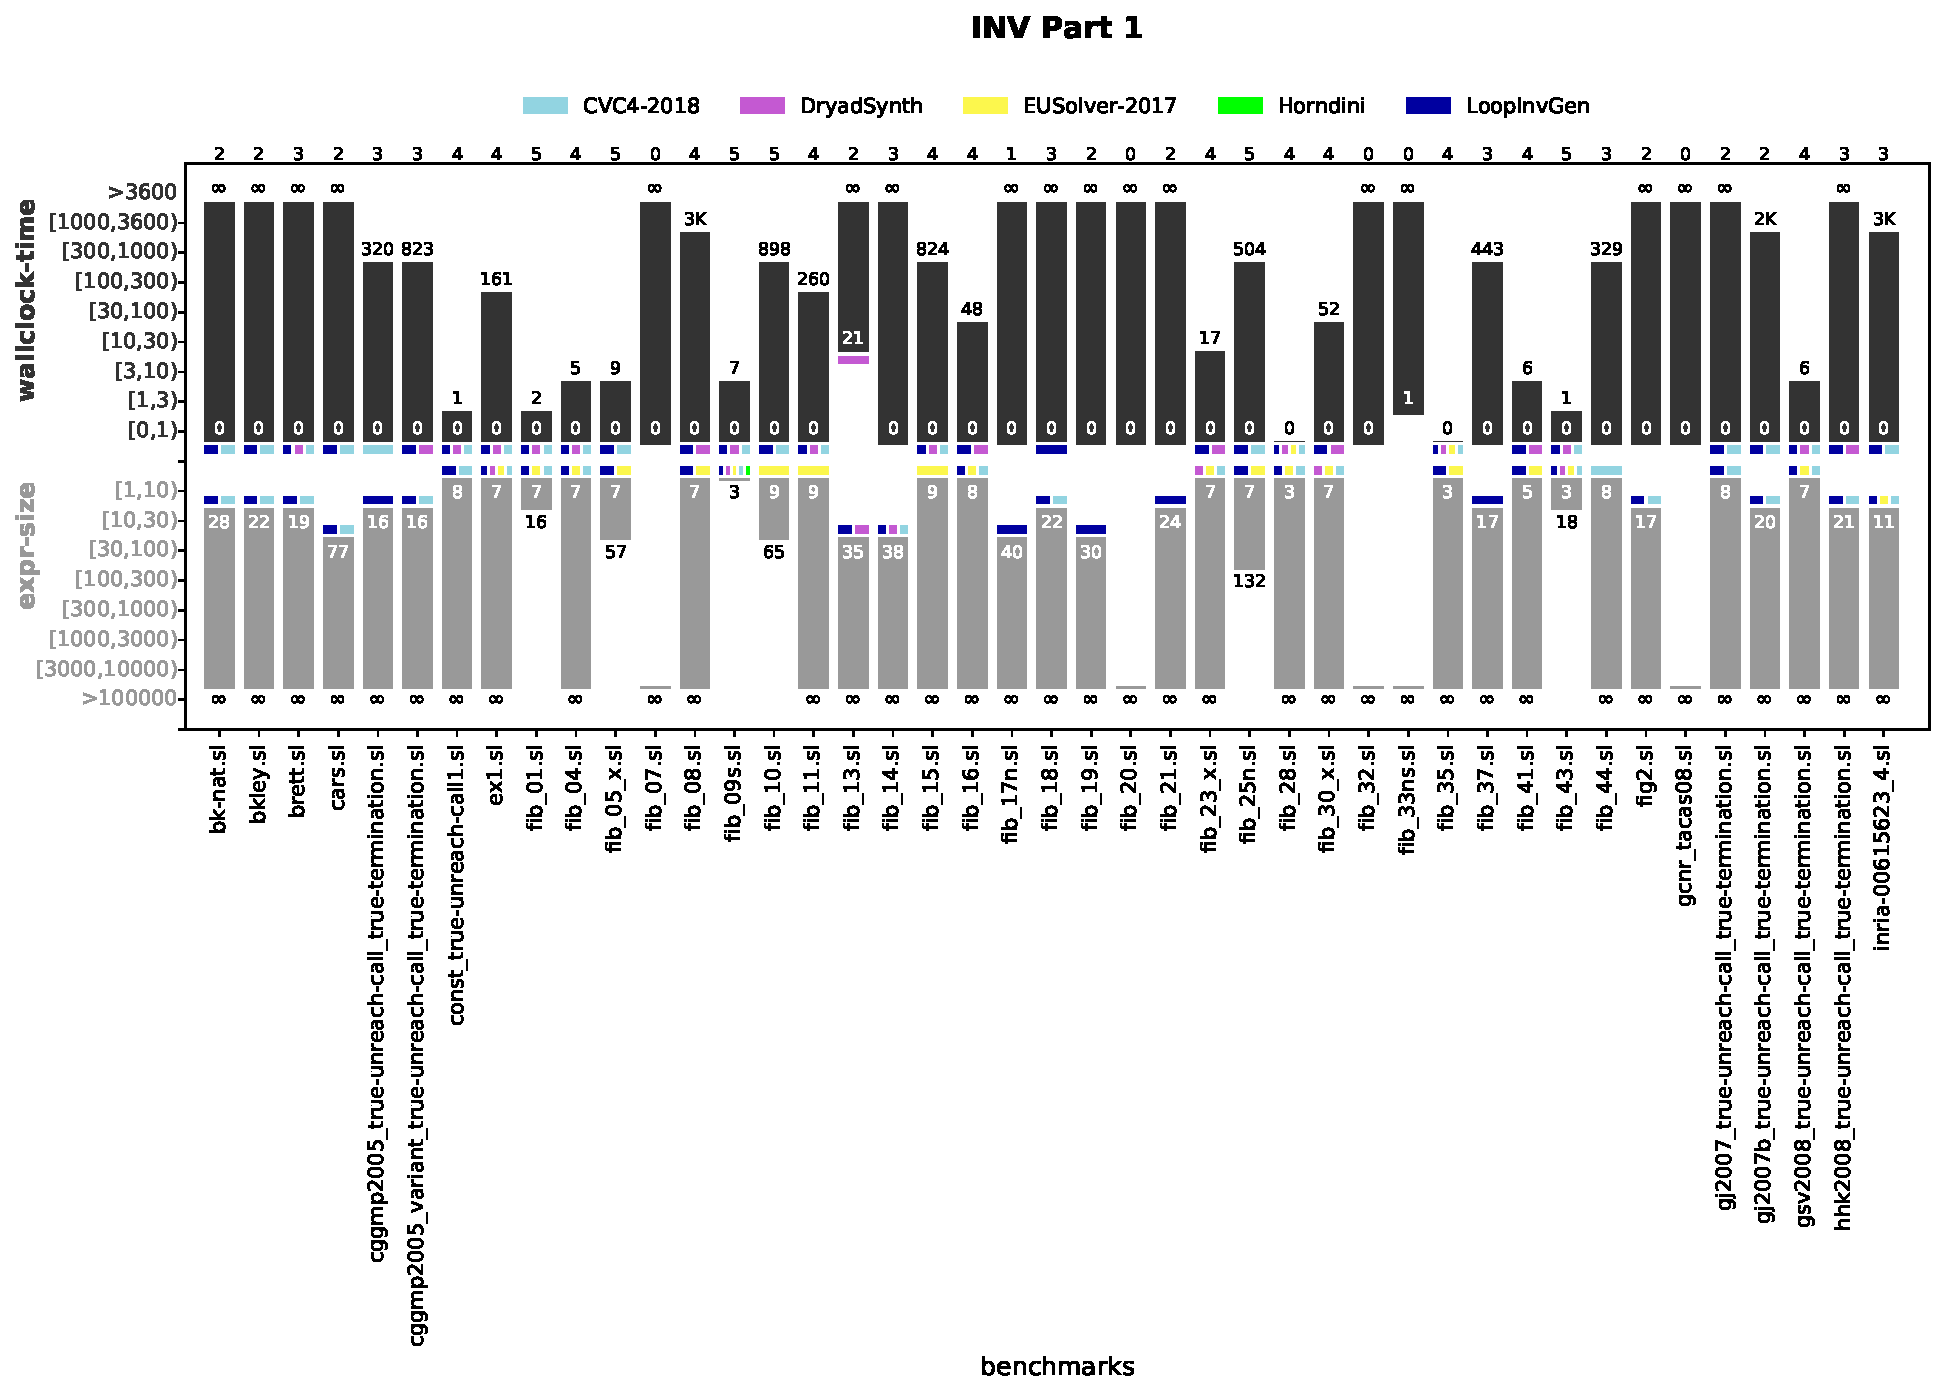
\includegraphics[width=10in]{figures/Inv1.pdf} \\[5mm]
				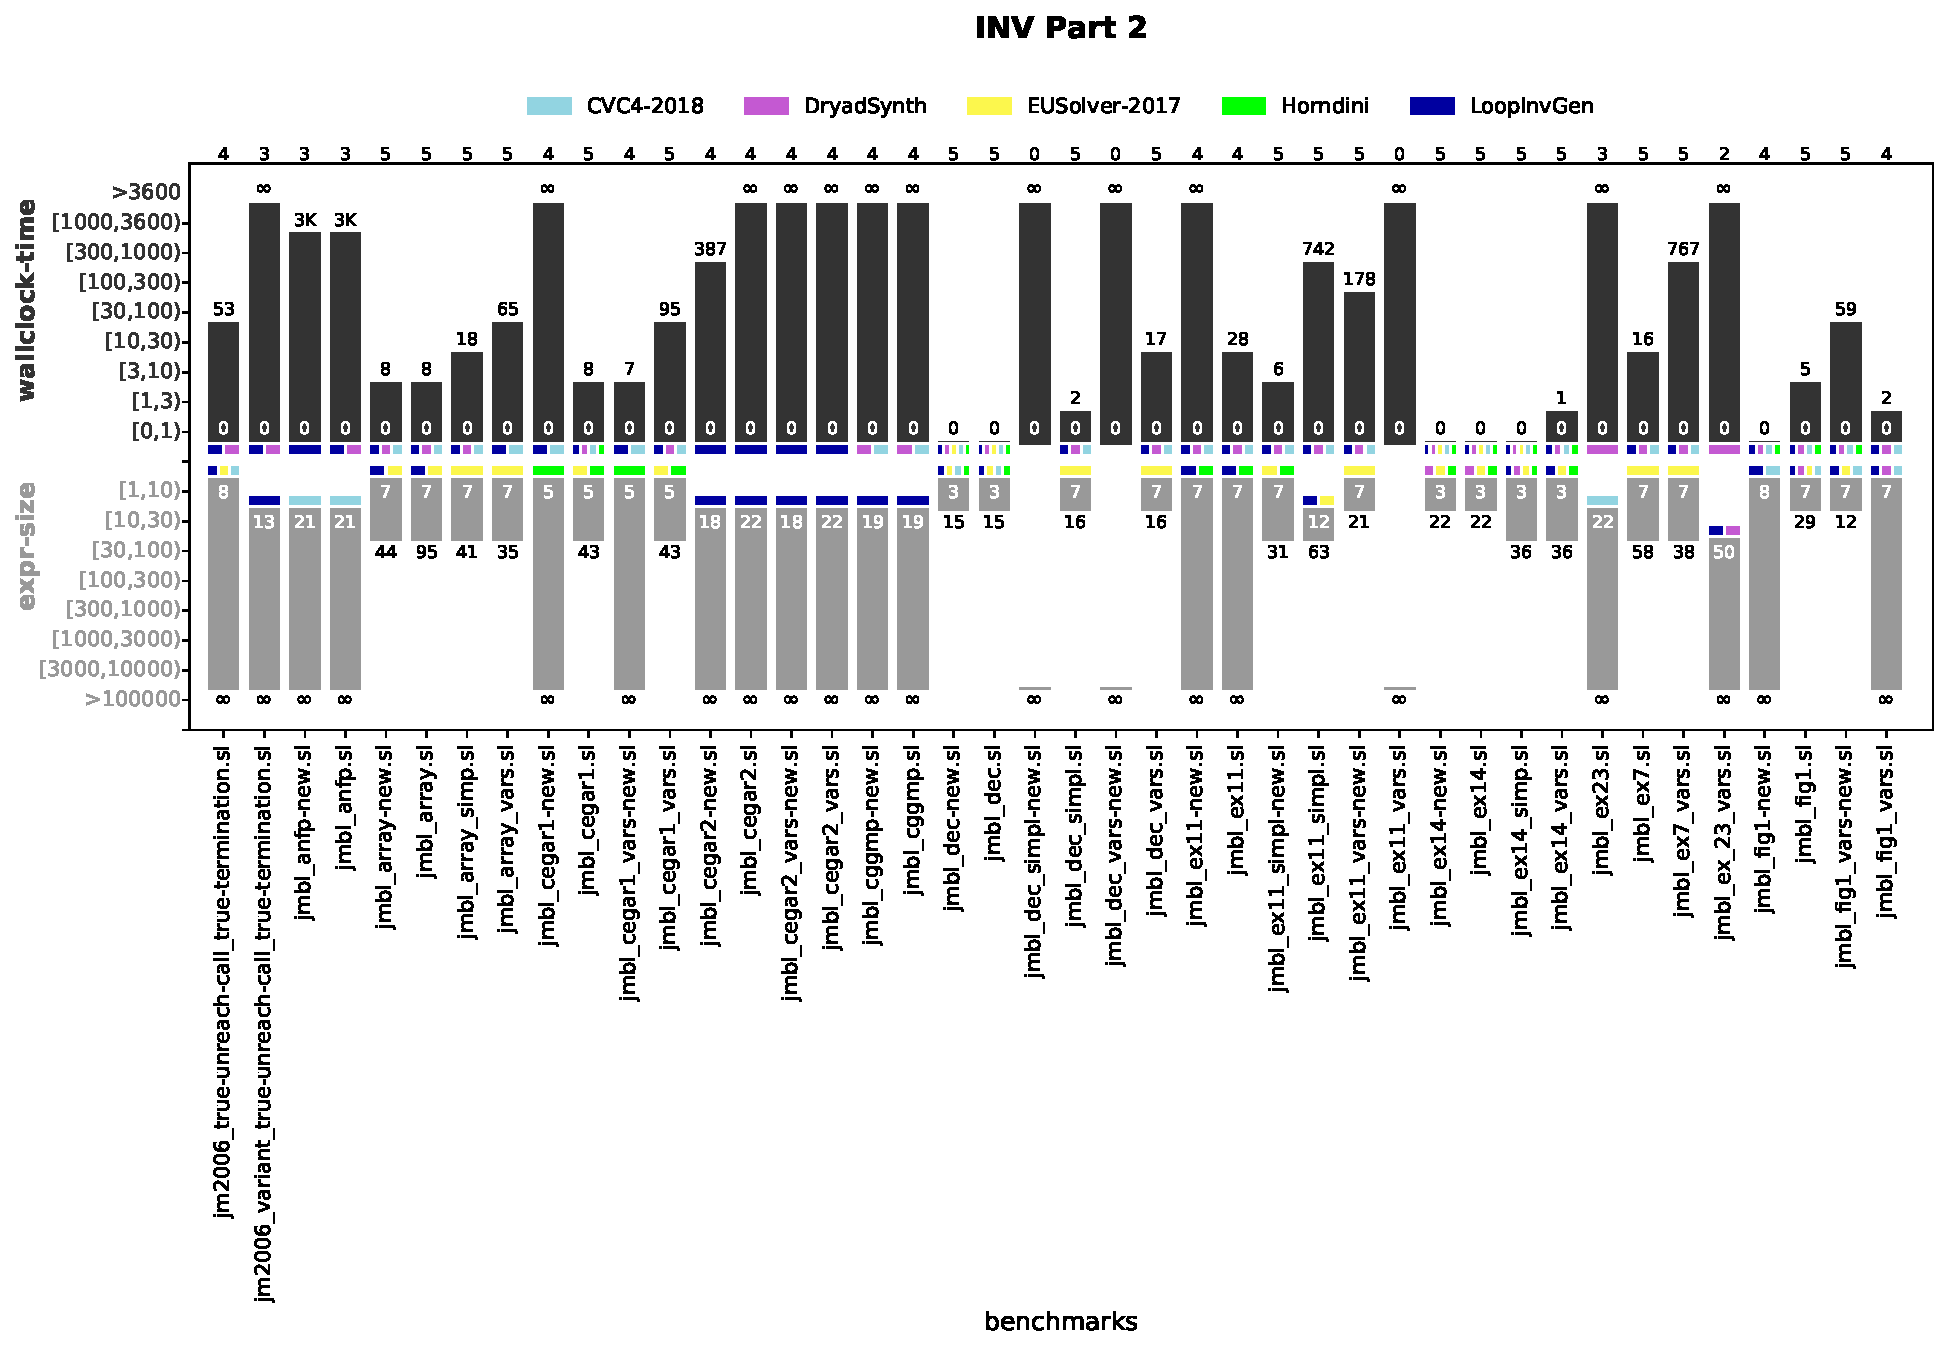
\includegraphics[width=10in]{figures/Inv2.pdf}
			\end{tabular}
	}}
	\caption{Evaluation of Invariant track benchmarks (Parts 1 \& 2).}
	\label{fig:inv-results-1}
\end{figure*}



\begin{figure*}
	\noindent\makebox[\textwidth]{
		\scalebox{0.6}{
			\begin{tabular}{c}
				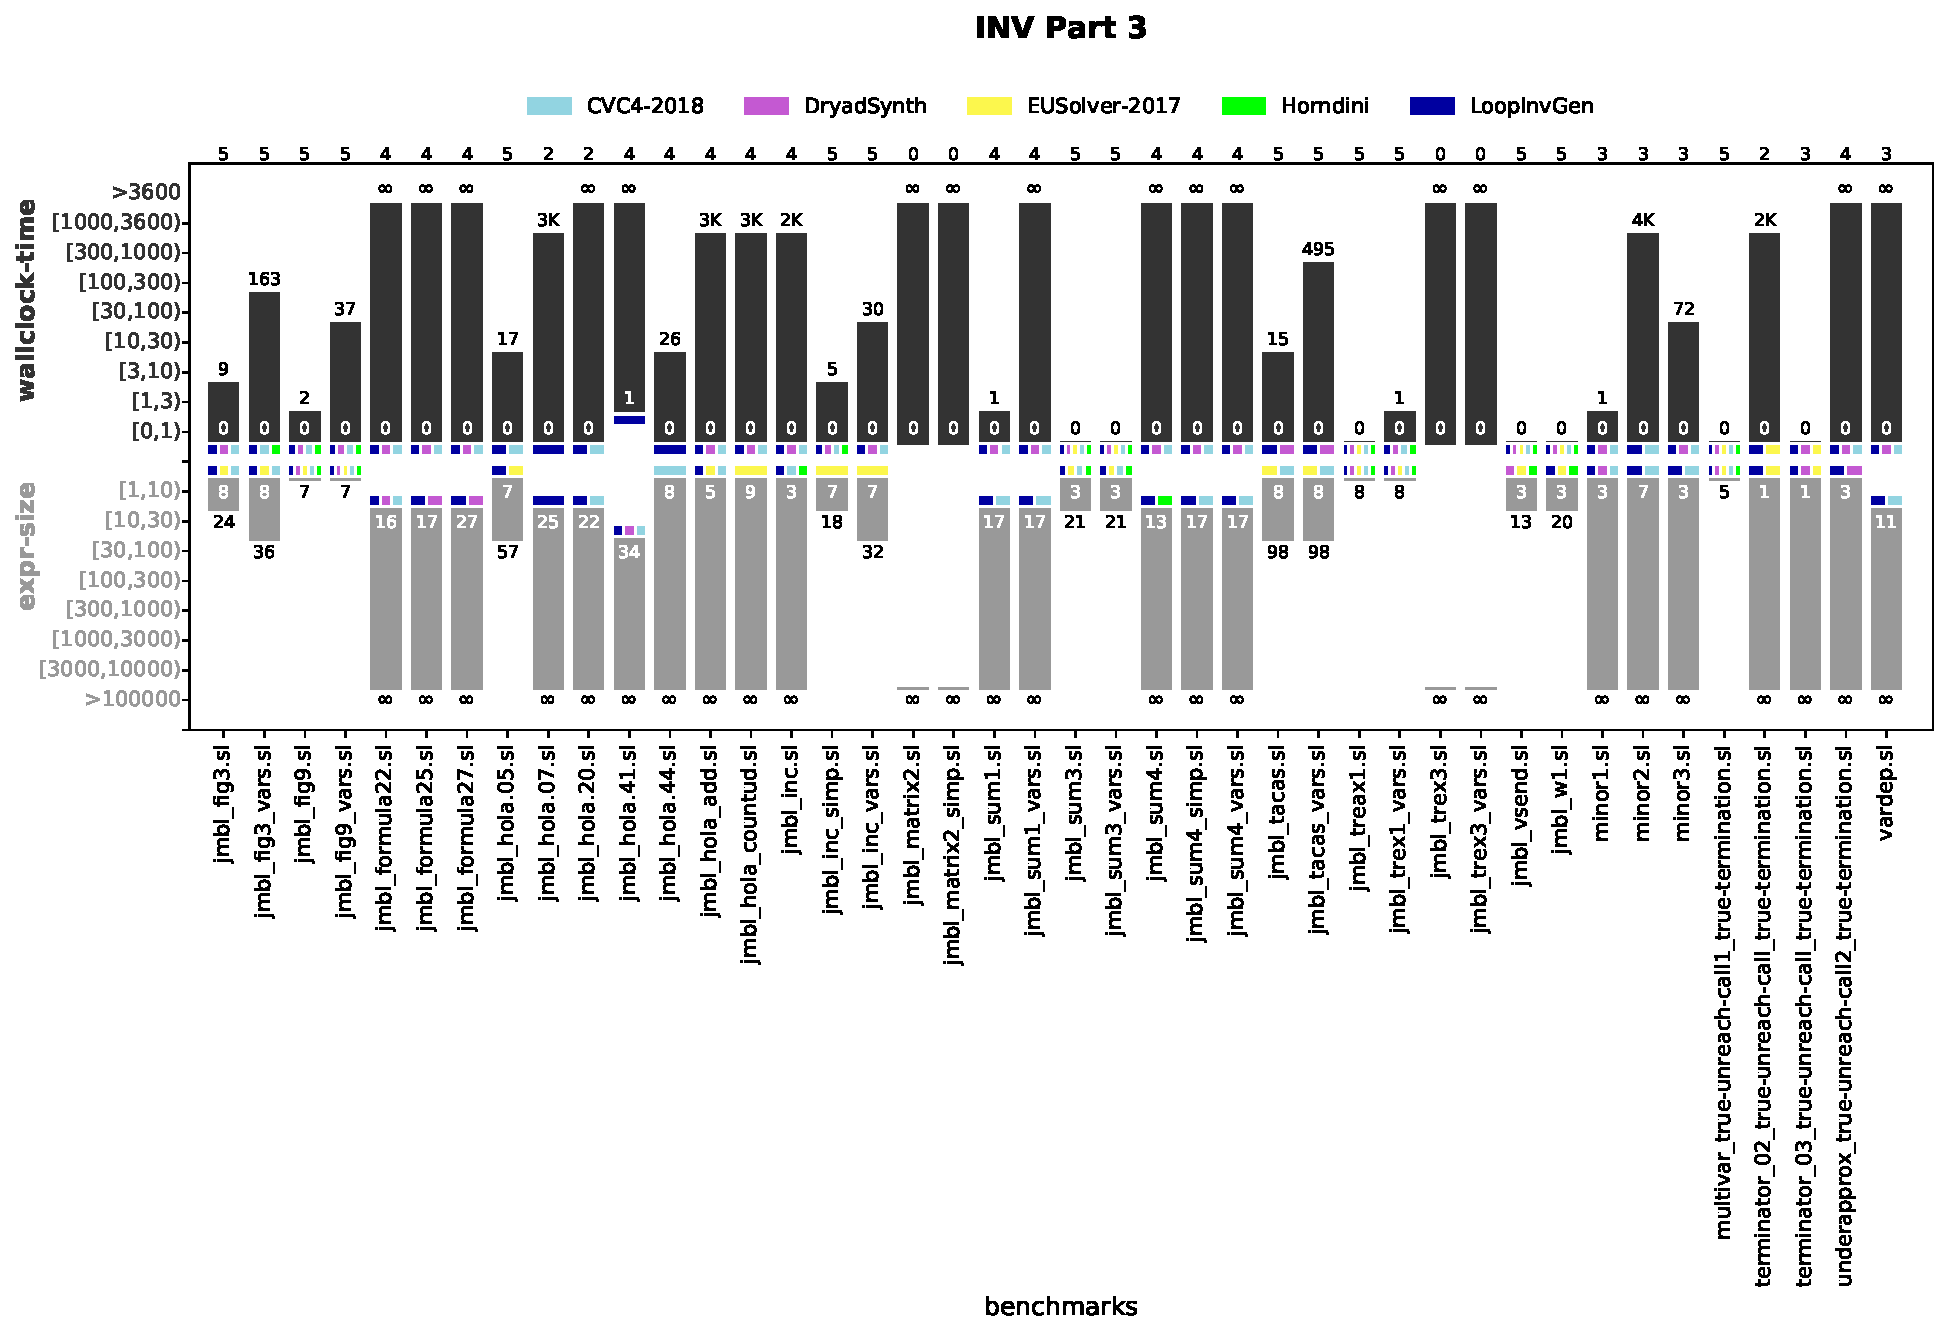
\includegraphics[width=10in]{figures/Inv3.pdf}
			\end{tabular}
		}}
	\caption{Evaluation of Invariant track benchmarks (Part 3).}
	\label{fig:inv-results-2}
\end{figure*}

\begin{figure*}
	\noindent\makebox[\textwidth]{
		\scalebox{0.6}{
			\begin{tabular}{c}
				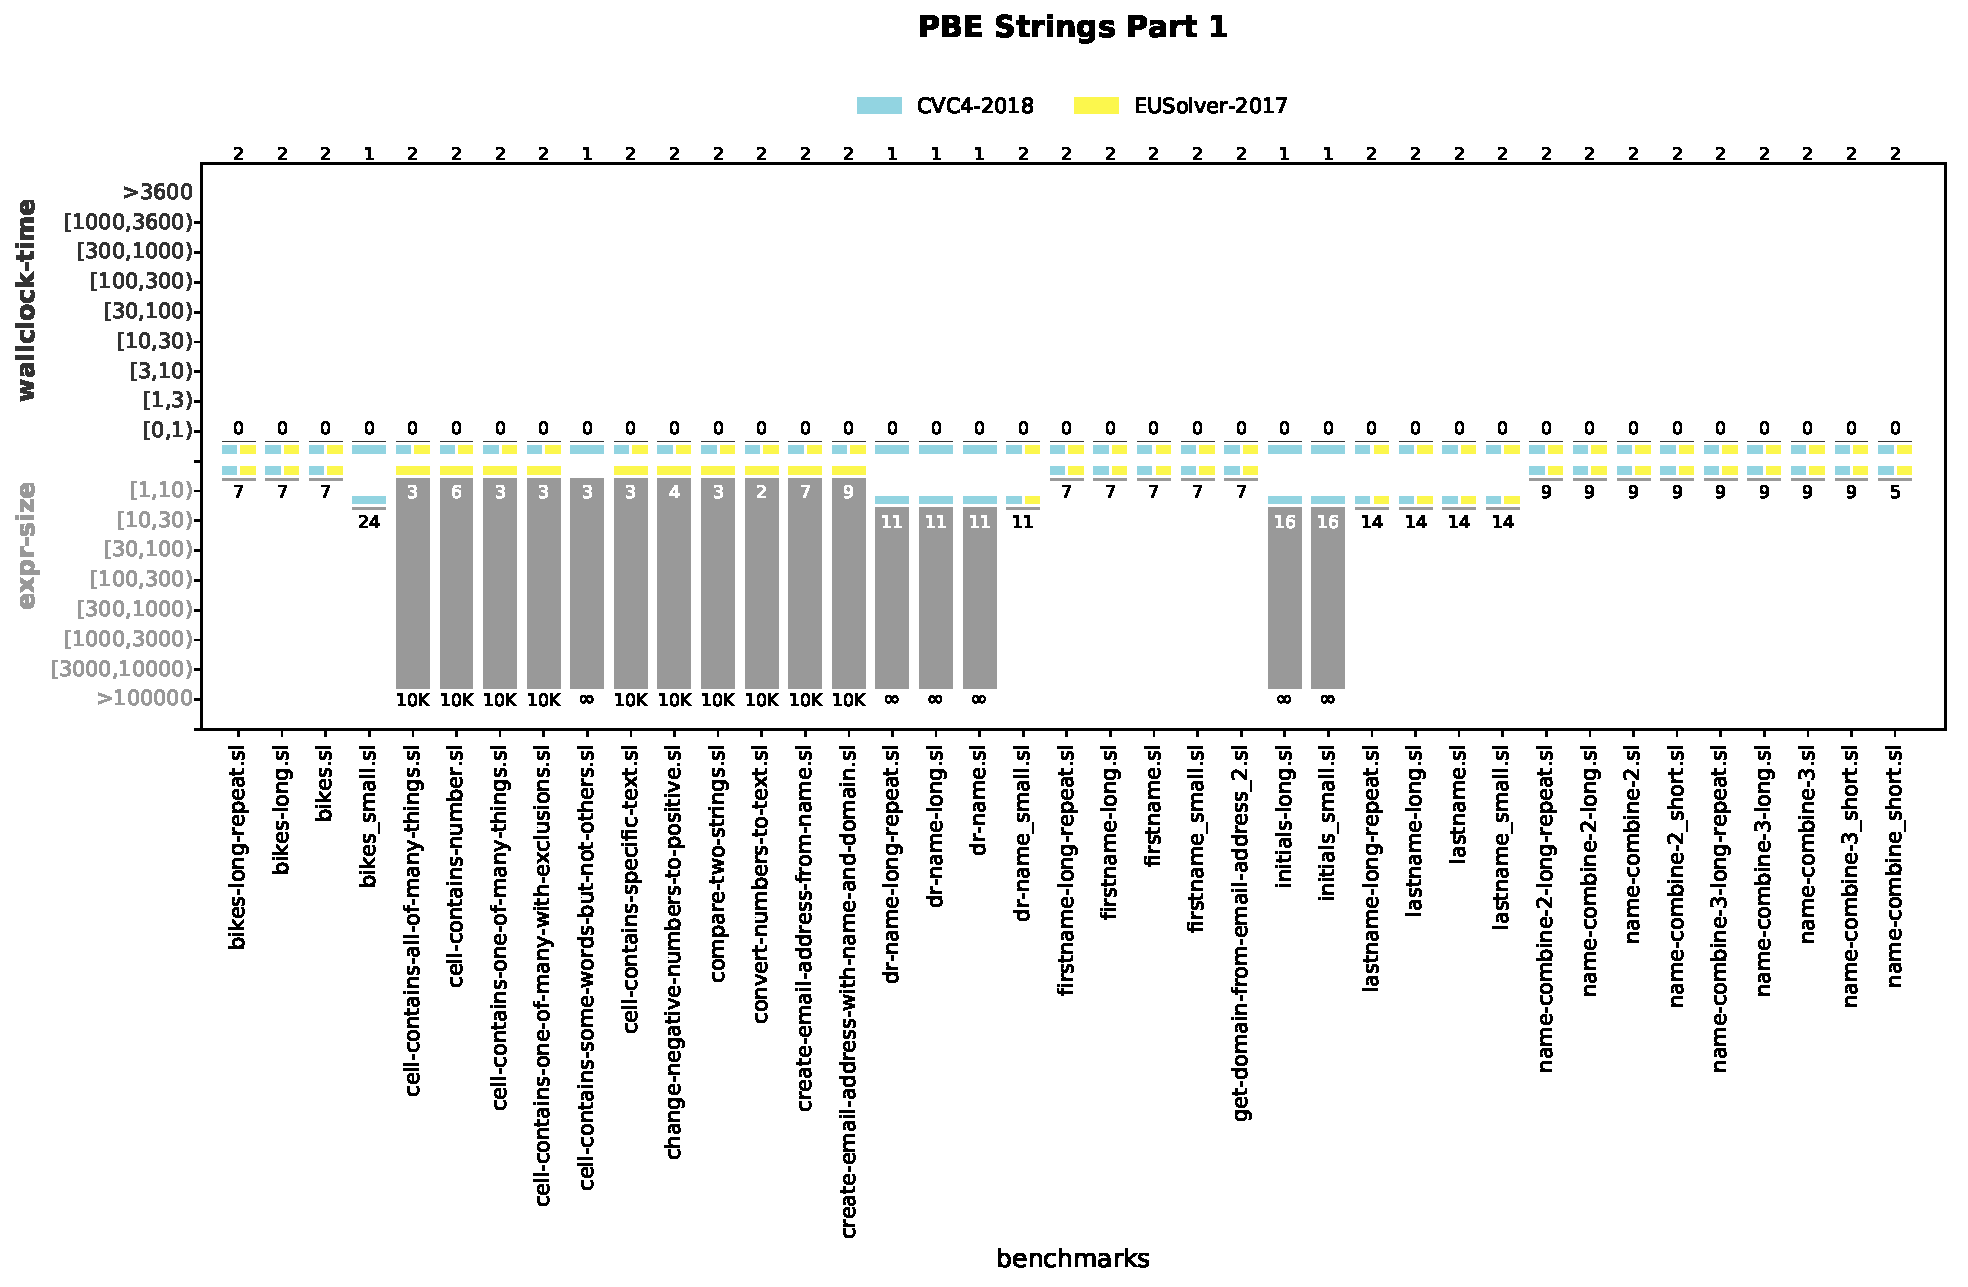
\includegraphics[width=10in]{figures/PBEStrings1.pdf} \\[3cm]
				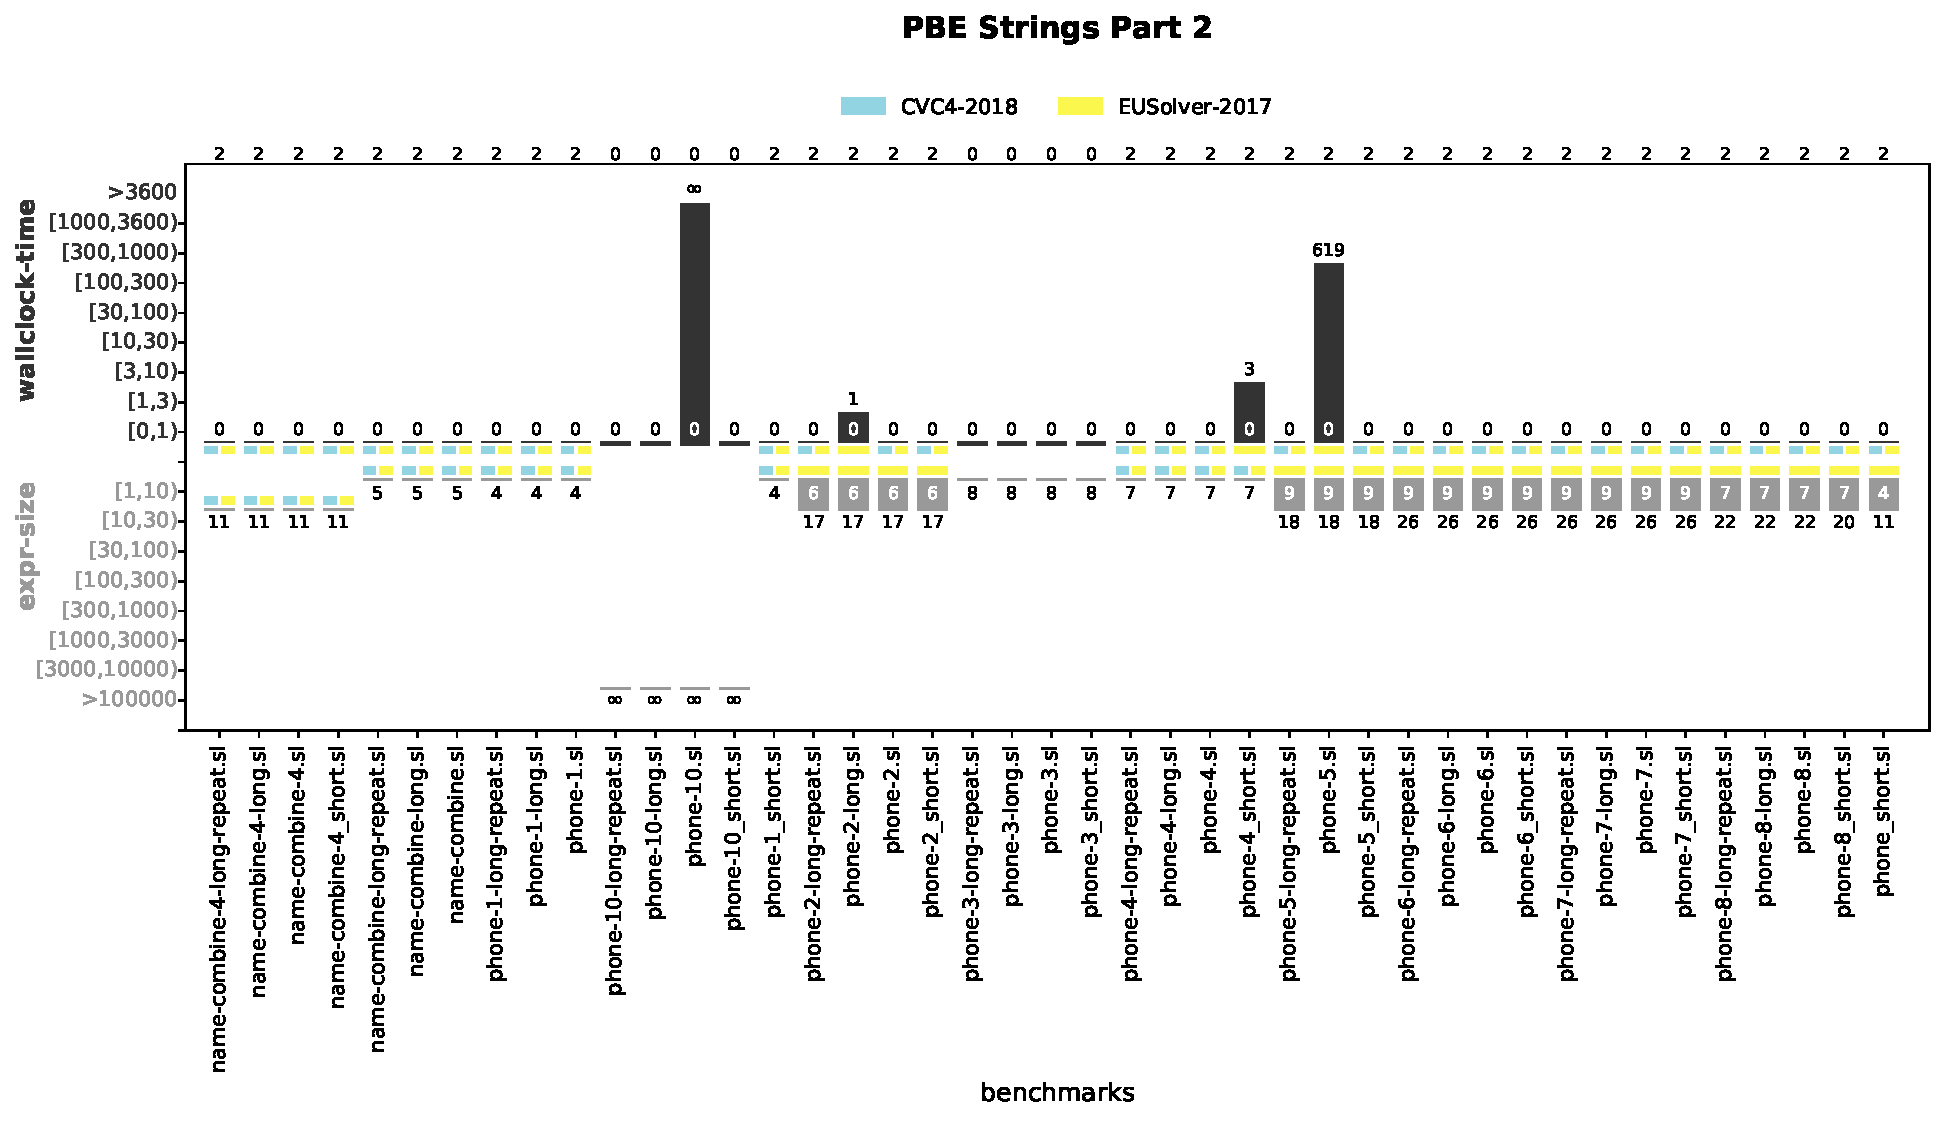
\includegraphics[width=10in]{figures/PBEStrings2.pdf} 
			\end{tabular}
		}}
	\caption{Evaluation of PBE Strings track benchmarks.}
	\label{fig:pbe-strings-results}
\end{figure*}


\section{Summary}
\label{sec:discussion}
This year's competition consisted of over 1600 benchmarks,
107 of which where contributed this year.
Five solvers competed this year, one of which was submitted by developers creating a tool for SyGuS-Comp for the first time.
All tools preformed remarkably, on both existing and new benchmarks.
In particular, \verify{65\%} of the new benchmarks were solved.

An impressive progress was shown this year in solving the strings benchmarks of the programing by example track.
Analyzing the features of benchmarks that are still hard to solve,
we see that these include those with either \verify{<features> ...}
%(i) multiple functions to synthesize or (ii) where the specification invokes the functions with different parameters or (iii) those that use the \emph{let} expression for specifying auxiliary variables, or (iv) the grammar is very general consisting of much more operators than needed, or (v) the specification is partial in the sense that the domain of semantic solutions is not a singleton.


\bibliographystyle{eptcs}
\bibliography{paper}

\end{document}